%Version 3 October 2023
%DIF LATEXDIFF DIFFERENCE FILE
%DIF DEL /Users/armanmohamadi/Documents/ChatGPT/Article/original_article/Paper.tex   Sat Feb 14 08:04:06 2026
%DIF ADD outputs/manuscript_preserved_revision/Paper.tex                             Wed Nov  4 14:27:39 2026
% See section 11 of the User Manual for version history
%
%%%%%%%%%%%%%%%%%%%%%%%%%%%%%%%%%%%%%%%%%%%%%%%%%%%%%%%%%%%%%%%%%%%%%%
%%                                                                 %%
%% Please do not use \input{...} to include other tex files.       %%
%% Submit your LaTeX manuscript as one .tex document.              %%
%%                                                                 %%
%% All additional figures and files should be attached             %%
%% separately and not embedded in the \TeX\ document itself.       %%
%%                                                                 %%
%%%%%%%%%%%%%%%%%%%%%%%%%%%%%%%%%%%%%%%%%%%%%%%%%%%%%%%%%%%%%%%%%%%%%

%%\documentclass[referee,sn-basic]{sn-jnl}% referee option is meant for double line spacing

%%=======================================================%%
%% to print line numbers in the margin use lineno option %%
%%=======================================================%%

%%\documentclass[lineno,sn-basic]{sn-jnl}% Basic Springer Nature Reference Style/Chemistry Reference Style

%%======================================================%%
%% to compile with pdflatex/xelatex use pdflatex option %%
%%======================================================%%

%%\documentclass[pdflatex,sn-basic]{sn-jnl}% Basic Springer Nature Reference Style/Chemistry Reference Style


%DIF 29c29
%DIF < %%Note: the following reference styles support Namedate and Numbered referencing. By default the style follows the most common style. To switch between the options you can add or remove “Numbered” in the optional parenthesis. 
%DIF -------
%%Note: the following reference styles support Namedate and Numbered referencing. By default the style follows the most common style. To switch between the options you can add or remove “Numbered” in the optional parenthesis.  %DIF > 
%DIF -------
%%The option is available for: sn-basic.bst, sn-vancouver.bst, sn-chicago.bst%  
 
%%\documentclass[sn-nature]{sn-jnl}% Style for submissions to Nature Portfolio journals
%%\documentclass[sn-basic]{sn-jnl}% Basic Springer Nature Reference Style/Chemistry Reference Style
\documentclass[sn-mathphys-num, Numbered]{sn-jnl}% Math and Physical Sciences Numbered Reference Style 
%%\documentclass[sn-mathphys-ay]{sn-jnl}% Math and Physical Sciences Author Year Reference Style
%%\documentclass[sn-aps]{sn-jnl}% American Physical Society (APS) Reference Style
%\documentclass[sn-vancouver,Numbered]{sn-jnl}% Vancouver Reference Style
%\documentclass[sn-apa]{sn-jnl}% APA Reference Style 
%%\documentclass[sn-chicago]{sn-jnl}% Chicago-based Humanities Reference Style

%%%% Standard Packages
%%<additional latex packages if required can be included here>

\usepackage{graphicx}%
\usepackage{multirow}%
\usepackage{amsmath,amssymb,amsfonts}%
\usepackage{amsthm}%
\usepackage{mathrsfs}%
\usepackage[title]{appendix}%
\usepackage[table]{xcolor}%
\usepackage{textcomp}%
\usepackage{manyfoot}%
\usepackage{booktabs}%
\usepackage{algorithm}%
\usepackage{algorithmicx}%
\usepackage{algpseudocode}%
\usepackage{listings}%
\usepackage{subcaption}
%DIF 59a59-60
\usepackage{pgfplots} %DIF > 
\pgfplotsset{compat=1.18} %DIF > 
\usepackage{tikz} %DIF >
\usetikzlibrary{positioning} %DIF >
%DIF -------
%%%%

%%%%%=============================================================================%%%%
%%%%  Remarks: This template is provided to aid authors with the preparation
%%%%  of original research articles intended for submission to journals published 
%%%%  by Springer Nature. The guidance has been prepared in partnership with 
%%%%  production teams to conform to Springer Nature technical requirements. 
%%%%  Editorial and presentation requirements differ among journal portfolios and 
%%%%  research disciplines. You may find sections in this template are irrelevant 
%%%%  to your work and are empowered to omit any such section if allowed by the 
%%%%  journal you intend to submit to. The submission guidelines and policies 
%%%%  of the journal take precedence. A detailed User Manual is available in the 
%%%%  template package for technical guidance.
%%%%%=============================================================================%%%%

%% as per the requirement new theorem styles can be included as shown below
\theoremstyle{thmstyleone}%
\newtheorem{theorem}{Theorem}%  meant for continuous numbers
%%\newtheorem{theorem}{Theorem}[section]% meant for sectionwise numbers
%% optional argument [theorem] produces theorem numbering sequence instead of independent numbers for Proposition
\newtheorem{proposition}[theorem]{Proposition}% 
%%\newtheorem{proposition}{Proposition}% to get separate numbers for theorem and proposition etc.

\theoremstyle{thmstyletwo}%
\newtheorem{example}{Example}%
\newtheorem{remark}{Remark}%

\theoremstyle{thmstylethree}%
\newtheorem{definition}{Definition}%

\raggedbottom
%%\unnumbered% uncomment this for unnumbered level heads

\setlength{\textfloatsep}{18pt plus 2pt minus 2pt} %DIF > 
\setlength{\intextsep}{16pt plus 2pt minus 2pt} %DIF > 
\setlength{\belowcaptionskip}{6pt} %DIF > 
\setlength{\belowdisplayskip}{14pt plus 2pt minus 2pt} %DIF > 
\setlength{\belowdisplayshortskip}{10pt plus 2pt minus 2pt} %DIF > 
%DIF PREAMBLE EXTENSION ADDED BY LATEXDIFF
%DIF UNDERLINE PREAMBLE %DIF PREAMBLE
\RequirePackage[normalem]{ulem} %DIF PREAMBLE
\RequirePackage{color}\definecolor{RED}{rgb}{1,0,0}\definecolor{BLUE}{rgb}{0,0,1} %DIF PREAMBLE
\providecommand{\DIFadd}[1]{{\protect\color{green!40!black}#1}} %DIF PREAMBLE
\providecommand{\DIFdel}[1]{}                      %DIF PREAMBLE
%DIF SAFE PREAMBLE %DIF PREAMBLE
\providecommand{\DIFaddbegin}{} %DIF PREAMBLE
\providecommand{\DIFaddend}{} %DIF PREAMBLE
\providecommand{\DIFdelbegin}{} %DIF PREAMBLE
\providecommand{\DIFdelend}{} %DIF PREAMBLE
\providecommand{\DIFmodbegin}{} %DIF PREAMBLE
\providecommand{\DIFmodend}{} %DIF PREAMBLE
%DIF FLOATSAFE PREAMBLE %DIF PREAMBLE
\providecommand{\DIFaddFL}[1]{\DIFadd{#1}} %DIF PREAMBLE
\providecommand{\DIFdelFL}[1]{\DIFdel{#1}} %DIF PREAMBLE
\providecommand{\DIFaddbeginFL}{} %DIF PREAMBLE
\providecommand{\DIFaddendFL}{} %DIF PREAMBLE
\providecommand{\DIFdelbeginFL}{} %DIF PREAMBLE
\providecommand{\DIFdelendFL}{} %DIF PREAMBLE
\newcommand{\DIFscaledelfig}{0.5}
%DIF HIGHLIGHTGRAPHICS PREAMBLE %DIF PREAMBLE
\RequirePackage{settobox} %DIF PREAMBLE
\RequirePackage{letltxmacro} %DIF PREAMBLE
\newsavebox{\DIFdelgraphicsbox} %DIF PREAMBLE
\newlength{\DIFdelgraphicswidth} %DIF PREAMBLE
\newlength{\DIFdelgraphicsheight} %DIF PREAMBLE
% store original definition of \includegraphics %DIF PREAMBLE
\LetLtxMacro{\DIFOincludegraphics}{\includegraphics} %DIF PREAMBLE
\newcommand{\DIFaddincludegraphics}[2][]{{\color{blue}\fbox{\DIFOincludegraphics[#1]{#2}}}} %DIF PREAMBLE
\newcommand{\DIFdelincludegraphics}[2][]{% %DIF PREAMBLE
\sbox{\DIFdelgraphicsbox}{\DIFOincludegraphics[#1]{#2}}% %DIF PREAMBLE
\settoboxwidth{\DIFdelgraphicswidth}{\DIFdelgraphicsbox} %DIF PREAMBLE
\settoboxtotalheight{\DIFdelgraphicsheight}{\DIFdelgraphicsbox} %DIF PREAMBLE
\scalebox{\DIFscaledelfig}{% %DIF PREAMBLE
\parbox[b]{\DIFdelgraphicswidth}{\usebox{\DIFdelgraphicsbox}\\[-\baselineskip] \rule{\DIFdelgraphicswidth}{0em}}\llap{\resizebox{\DIFdelgraphicswidth}{\DIFdelgraphicsheight}{% %DIF PREAMBLE
\setlength{\unitlength}{\DIFdelgraphicswidth}% %DIF PREAMBLE
\begin{picture}(1,1)% %DIF PREAMBLE
\thicklines\linethickness{2pt} %DIF PREAMBLE
{\color[rgb]{1,0,0}\put(0,0){\framebox(1,1){}}}% %DIF PREAMBLE
{\color[rgb]{1,0,0}\put(0,0){\line( 1,1){1}}}% %DIF PREAMBLE
{\color[rgb]{1,0,0}\put(0,1){\line(1,-1){1}}}% %DIF PREAMBLE
\end{picture}% %DIF PREAMBLE
}\hspace*{3pt}}} %DIF PREAMBLE
} %DIF PREAMBLE
\LetLtxMacro{\DIFOaddbegin}{\DIFaddbegin} %DIF PREAMBLE
\LetLtxMacro{\DIFOaddend}{\DIFaddend} %DIF PREAMBLE
\LetLtxMacro{\DIFOdelbegin}{\DIFdelbegin} %DIF PREAMBLE
\LetLtxMacro{\DIFOdelend}{\DIFdelend} %DIF PREAMBLE
\DeclareRobustCommand{\DIFaddbegin}{\DIFOaddbegin \let\includegraphics\DIFaddincludegraphics} %DIF PREAMBLE
\DeclareRobustCommand{\DIFaddend}{\DIFOaddend \let\includegraphics\DIFOincludegraphics} %DIF PREAMBLE
\DeclareRobustCommand{\DIFdelbegin}{\DIFOdelbegin \let\includegraphics\DIFdelincludegraphics} %DIF PREAMBLE
\DeclareRobustCommand{\DIFdelend}{\DIFOaddend \let\includegraphics\DIFOincludegraphics} %DIF PREAMBLE
\LetLtxMacro{\DIFOaddbeginFL}{\DIFaddbeginFL} %DIF PREAMBLE
\LetLtxMacro{\DIFOaddendFL}{\DIFaddendFL} %DIF PREAMBLE
\LetLtxMacro{\DIFOdelbeginFL}{\DIFdelbeginFL} %DIF PREAMBLE
\LetLtxMacro{\DIFOdelendFL}{\DIFdelendFL} %DIF PREAMBLE
\DeclareRobustCommand{\DIFaddbeginFL}{\DIFOaddbeginFL \let\includegraphics\DIFaddincludegraphics} %DIF PREAMBLE
\DeclareRobustCommand{\DIFaddendFL}{\DIFOaddendFL \let\includegraphics\DIFOincludegraphics} %DIF PREAMBLE
\DeclareRobustCommand{\DIFdelbeginFL}{\DIFOdelbeginFL \let\includegraphics\DIFdelincludegraphics} %DIF PREAMBLE
\DeclareRobustCommand{\DIFdelendFL}{\DIFOaddendFL \let\includegraphics\DIFOincludegraphics} %DIF PREAMBLE
%DIF COLORLISTINGS PREAMBLE %DIF PREAMBLE
\RequirePackage{listings} %DIF PREAMBLE
\RequirePackage{color} %DIF PREAMBLE
\lstdefinelanguage{DIFcode}{ %DIF PREAMBLE
%DIF DIFCODE_UNDERLINE %DIF PREAMBLE
  moredelim=[il][\color{red}\sout]{\%DIF\ <\ }, %DIF PREAMBLE
  moredelim=[il][\color{blue}\uwave]{\%DIF\ >\ } %DIF PREAMBLE
} %DIF PREAMBLE
\lstdefinestyle{DIFverbatimstyle}{ %DIF PREAMBLE
	language=DIFcode, %DIF PREAMBLE
	basicstyle=\ttfamily, %DIF PREAMBLE
	columns=fullflexible, %DIF PREAMBLE
	keepspaces=true %DIF PREAMBLE
} %DIF PREAMBLE
\lstnewenvironment{DIFverbatim}{\lstset{style=DIFverbatimstyle}}{} %DIF PREAMBLE
\lstnewenvironment{DIFverbatim*}{\lstset{style=DIFverbatimstyle,showspaces=true}}{} %DIF PREAMBLE
%DIF END PREAMBLE EXTENSION ADDED BY LATEXDIFF

\begin{document}

\title[Article Title]{User Next Click Prediction Using Machine Learning for UX Analysis}

%%=============================================================%%
%% GivenName	-> \fnm{Joergen W.}
%% Particle	-> \spfx{van der} -> surname prefix
%% FamilyName	-> \sur{Ploeg}
%% Suffix	-> \sfx{IV}
%% \author*[1,2]{\fnm{Joergen W.} \spfx{van der} \sur{Ploeg} 
%%  \sfx{IV}}\email{iauthor@gmail.com}
%%=============================================================%%


%
%\author[1]{\fnm{Arman} \sur{MohammadiAsl}}\email{ar.mohammadi@sci.ui.ac.ir}
%
%\author*[1]{\fnm{Mohsen} \sur{Alambardar Meybodi}}\email{m.alambardar@sci.ui.ac.ir}
%%\equalcont{These authors contributed equally to this work.}
%
%\author[2]{\fnm{Marjan} \sur{Kaedi}}\email{kaedi@eng.ui.ac.ir}
%%\equalcont{These authors contributed equally to this work.}
%
%\affil*[1]{\orgdiv{Department of Applied Mathematics and Computer Science}, \orgname{Faculty of Mathematics and Statistics, University of Isfahan}, \orgaddress{\city{Isfahan}, \postcode{81746-73441}, \country{Iran}}}
%
%\affil[2]{\orgdiv{Faculty of Computer Engineering}, \orgname{University of Isfahan}, \orgaddress{\city{Isfahan}, \postcode{81746-73441}, \country{Iran}}}
%

%%==================================%%
%% Sample for unstructured abstract %%
%%==================================%%

\DIFdelbegin %DIFDELCMD < \abstract{
%DIFDELCMD < 		Modeling user click sequences in a mobile application can significantly enhance the understanding of user experience by analyzing behavior across different application pages. By predicting clickable elements that users are likely to interact with, this modeling helps identify possible interface improvements, ultimately enhancing overall user experience and satisfaction.
%DIFDELCMD < 		This research aims to improve productivity and quality in conducting user experience tests, leading to better software usability and increased user satisfaction. As part of this contribution,  and after analyzing related works and evaluating their strengths and weaknesses, over 35,000 click events from 50 users interacting with a mobile application designed for employee recognition were collected and preprocessed.
%DIFDELCMD < 		The dataset includes User IDs, Clickable Elements, Pages, and Click Times, which were provided as input to the model. The final output is User Next Click Prediction (UNCP) using Long Short-Term Memory (LSTM) , Transformer ,and achieved an accuracy of 88\% with the LSTM model and 86\% with the Transformer model using the `Top-3 Accuracy` metric. Additionally, using the `Top-1 Accuracy` metric, an accuracy of 74\% was achieved with the LSTM model and 67\% with the Transformer model.
%DIFDELCMD < 		}
%DIFDELCMD < 
%%%
\DIFdelend \DIFaddbegin \abstract{
Modeling click sequences in a mobile application can support the analysis of user behavior across interface pages and help guide future UX evaluation. This study evaluates next-click prediction in an enterprise application using 46,194 recorded click events in 4,223 sequences. Complete User IDs are assigned to training, validation, and test partitions before prefix--target examples are generated. We compare the proposed validation-selected UNCP 5 with LSTM and Transformer reference models under the same user-disjoint protocol. Mean Top-3 accuracy over three seeds is 85.09\% for UNCP 5, 78.00\% for LSTM, and 71.92\% for Transformer. These results demonstrate next-click prediction under the specified evaluation conditions; potential UX improvements require prospective user testing.
}
\DIFaddend 

%%================================%%
%% Sample for structured abstract %%
%%================================%%

% \abstract{\textbf{Purpose:} The abstract serves both as a general introduction to the topic and as a brief, non-technical summary of the main results and their implications. The abstract must not include subheadings (unless expressly permitted in the journal's Instructions to Authors), equations or citations. As a guide the abstract should not exceed 200 words. Most journals do not set a hard limit however authors are advised to check the author instructions for the journal they are submitting to.
% 
% \textbf{Methods:} The abstract serves both as a general introduction to the topic and as a brief, non-technical summary of the main results and their implications. The abstract must not include subheadings (unless expressly permitted in the journal's Instructions to Authors), equations or citations. As a guide the abstract should not exceed 200 words. Most journals do not set a hard limit however authors are advised to check the author instructions for the journal they are submitting to.
% 
% \textbf{Results:} The abstract serves both as a general introduction to the topic and as a brief, non-technical summary of the main results and their implications. The abstract must not include subheadings (unless expressly permitted in the journal's Instructions to Authors), equations or citations. As a guide the abstract should not exceed 200 words. Most journals do not set a hard limit however authors are advised to check the author instructions for the journal they are submitting to.
% 
% \textbf{Conclusion:} The abstract serves both as a general introduction to the topic and as a brief, non-technical summary of the main results and their implications. The abstract must not include subheadings (unless expressly permitted in the journal's Instructions to Authors), equations or citations. As a guide the abstract should not exceed 200 words. Most journals do not set a hard limit however authors are advised to check the author instructions for the journal they are submitting to.}

%\keywords{keyword1, Keyword2, Keyword3, Keyword4}
\keywords{User Experience, User Modeling, Machine Learning, Click Models, Neural Networks.}

%%\pacs[JEL Classification]{D8, H51}

%%\pacs[MSC Classification]{35A01, 65L10, 65L12, 65L20, 65L70}

\maketitle


\section{Introduction}

\label{sec:intro}
User interaction behavior on smart mobile devices typically involves a sequence of taps or clicks\footnote{In this study, the term  \textit{click} is used instead of \textit{tap} to refer to interactions on the mobile application screen.} on touch-screen interface elements, resulting in a series of screen state transitions in response to these actions \cite{bohmer2011falling}. Predicting the next user click through machine learning models opens up new possibilities for enhancing user experience. For instance, interface elements can be reordered based on user interaction frequency, thereby improving efficiency and speeding up task completion. Furthermore, Adaptive User Interfaces (AUIs) can be dynamically activated to personalize the layout and make the interface more intuitive for future use \cite{parate2013practical}. An AUI adapts the arrangement of UI elements to the user's preferences or behavior patterns. This means components such as surveys, fund transfers, settings, and events on a page can be reordered either by the user or automatically based on usage frequency \cite{findlater2009ephemeral, tanvir2011improving}.

Numerous studies have focused on modeling user click behavior across domains such as mobile interaction \cite{lee2018click}, web navigation \cite{mao2018constructing}, advertising \cite{liu2015convolutional}, news consumption \cite{wu2019neural}, and e-commerce. Several works \cite{tanvir2011improving, browne2016adaptive, bohmer2011falling} have specifically explored user performance prediction at the application level. Zhou and Li \cite{zhou2021large} investigated computational modeling of click behavior as a foundation for adaptive UI systems. Their work focused on predicting the next UI element a user is likely to click. They developed LSTM- and Transformer-based learning models trained on user click data, taking into account click history, screen content, and current time to accurately forecast the next user action.


\textbf{Our Contribution:}
The main contributions of this study are summarized as follows:
\begin{itemize}
	\item {Model comparison:} Evaluation of \DIFdelbegin \DIFdel{LSTM and Transformermodels for user click sequence prediction using real-world enterprise app data}\DIFdelend \DIFaddbegin \DIFadd{transparent baselines, LSTM, GRU, Transformer, and six UNCP variants on the same held-out-user partition; the variants and their component combinations are identified in the result tables}\DIFaddend .

	\item {Real dataset:} \DIFdelbegin \DIFdel{Collection and preprocessing of over 35}\DIFdelend \DIFaddbegin \DIFadd{Analysis of 46}\DIFaddend {,}\DIFdelbegin \DIFdel{000 click events from 50 users; achieving 88\% top-3 and 74\% top-1 accuracy with LSTM}\DIFdelend \DIFaddbegin \DIFadd{194 click events in 4}{\DIFadd{,}}\DIFadd{223 sequences from 52 recorded User IDs, with complete User IDs held out from model fitting and preprocessing}\DIFaddend .

	\item {UX techniques:} \DIFdelbegin \DIFdel{Application of click-driven UX evaluation methods, including first-click testing and }\DIFdelend \DIFaddbegin \DIFadd{Use of predicted click rankings to identify possible UX improvements for evaluation in controlled }\DIFaddend usability studies.

	\item {\DIFdelbegin \DIFdel{Practical integration}\DIFdelend \DIFaddbegin \DIFadd{Decision support}\DIFaddend :} \DIFdelbegin \DIFdel{Bridging deep learning with UX design processes to automate and enhance enterprise mobile UI/UX workflows}\DIFdelend \DIFaddbegin \DIFadd{Examination of how predicted click rankings may help prioritize interface flows and possible design improvements for later UX investigation; efficiency and usability effects are not measured in this study}\DIFaddend .
\end{itemize}




\section{ Related Work}

In recent years, extensive research has been conducted on modeling user interactions and enhancing user experience through predictive systems. In this section, we review key studies that have contributed to this area.



%Previous works have shown that mobile user behaviors are influenced by various factors.


Baeza-Yates et al.~\cite{bohmer2011falling} proposed a predictive framework that identifies the next mobile application a user is likely to engage with. Their model utilizes a set of contextual features to predict the upcoming app interaction and subsequently reorganizes the app\DIFdelbegin \DIFdel{?}\DIFdelend \DIFaddbegin \DIFadd{'}\DIFaddend s menu layout based on the frequency of user access, thereby offering a more personalized experience.  Chen et al.~\cite{chen2019behavior} made significant advancements in predicting click-through rates (CTR) in Taobao's recommendation system by employing deep learning techniques. They introduced a Transformer-based recommendation model that represents user and item features as embedded vectors. These vectors are processed through a multi-layer fully connected neural network to estimate the likelihood of a user clicking on a specific item. Qin et al.~\cite{qin2020user} addressed user interest modeling by employing sequential behavior analysis in mobile applications. Their approach first selects relevant user actions from historical interaction sequences using information retrieval techniques, and then feeds them into a deep learning model for CTR prediction. This combination of retrieval-based filtering and deep learning improved the model's capacity to capture nuanced user preferences over time.

Yang et al. \cite{yang2020measuring} simulated user experience in the process of running a mobile app in their proposed model using machine learning. They used predicted app pages with the effect of time on element selection (see figure \ref{fig:PagesAndTimes}) to train neural networks, which were formed from click information of all users during a specific task process. Zhou and Li \cite{zhou2021large}, researchers at Google, designed a deep learning model based on Transformer using a dataset obtained from user interactions with a mobile application. This model predicts the next element that the user is most likely to click on, based on the user's click history and user interface information (see figure \ref{fig:examplecontacts}).
Wu et al. \cite{wu2023screen} concentrate on understanding the functionality of user interface elements. This method enables better analysis by mapping UI elements to previous examples, incorporating their semantic properties, appearance, text, and how they function. The model is used for generating in-app tutorials, searching for UI elements, and testing them. For example, this algorithm can identify that a UI element on a page is a button with the text `Login` or a text field with the text `Sign Up`.

Sun et al. \cite{sun2022meta} introduced a new GUI-based architecture (GUITOD) that is capable of directly interacting with software using graphical tools instead of complex textual commands. The operations performed include clicking on buttons, text fields, search fields, and similar elements. Ultimately, by clicking on these elements, actions are carried out based on the scenario and user flow. Additionally, it is used for training dialogue models in mobile applications. This model also predicts the next action of the user. It is widely used for performing specific tasks such as hotel reservations, calendar scheduling, and online shopping. Wu et al.\cite{wu2023never} trained machine learning models to predict semantic information about user interfaces to make mobile apps more accessible and automated. They introduced a Never-ending UI Learner model, which automatically extracts real apps by interacting with UI elements. This model helps improve the understanding of UI elements in the app. Feng et al.\cite{feng2023video2action} have made mobile app tutorial videos a popular method for users to learn various features. To make these videos easily understandable for users, video creators need to annotate different actions in the video. They introduced an approach called Video2Action, based on image processing and deep learning, which automatically predicts and highlights the click locations in the video. Feng et al.\cite{feng2024mud} introduced a novel approach to automatically extract UI data from Android apps using Large Language Models (LLMs). This model is used for UI modeling and element identification. Zhou et al.\cite{zhou2024encode} proposed a two-stage long-term sequence modeling approach, consisting of offline extraction and online inference, which is used to familiarize with user interests for predicting associations with target items.

\DIFdelbegin \DIFdel{As reviewed in our Related Work section, none of the prior studies?including Baeza-Yates }\DIFdelend \DIFaddbegin \DIFadd{Related work on intelligent optimization provides additional systems context. Addula }\DIFaddend et al.\DIFdelbegin \DIFdel{\mbox{%DIFAUXCMD
\cite{bohmer2011falling}}\hskip0pt%DIFAUXCMD
, Yang et al. \mbox{%DIFAUXCMD
\cite{yang2020measuring}}\hskip0pt%DIFAUXCMD
, Sun }\DIFdelend \DIFaddbegin \DIFadd{~\mbox{%DIFAUXCMD
\cite{addula2024kookaburra} }\hskip0pt%DIFAUXCMD
proposed a hybrid Kookaburra--Pelican optimization approach for dynamic cloud load balancing, targeting improved workload distribution and resource utilization. Although that study addresses infrastructure optimization rather than next-click prediction, it illustrates how hybrid optimization can support adaptive system decisions. We cite it as broader background only, not as evidence for predictive accuracy or UX improvement in the present study.
}

\DIFadd{Human-centered AI is also relevant when predictive systems are deployed in workplace settings. Meduri }\DIFaddend et al.\DIFdelbegin \DIFdel{\mbox{%DIFAUXCMD
\cite{sun2022meta}}\hskip0pt%DIFAUXCMD
, and Zhou and Li \mbox{%DIFAUXCMD
\cite{zhou2021large}}\hskip0pt%DIFAUXCMD
?have incorporated UX testing methods to improve user experience or proposed an intelligent assistant to support }\DIFdelend \DIFaddbegin \DIFadd{~\mbox{%DIFAUXCMD
\cite{meduri2024human} }\hskip0pt%DIFAUXCMD
studied how personalization, employee training, and feedback shape the effects of AI-supported workload management and emphasized that human-centered implementation matters beyond model performance. We cite this work as contextual motivation for careful, human-centered UX analysis; it is not used as evidence that the present next-click model improves employee well-being or usability.
}


\DIFadd{As reviewed in our Related Work section, prior studies have examined next-action prediction and adaptive interfaces. The present study contributes a leakage-aware comparison of next-click models on an enterprise clickstream and explores predicted rankings as a possible decision-support signal for }\DIFaddend UX researchers. \DIFdelbegin \DIFdel{Our model uniquely leverages user click data not only for predictive modeling but also to automate UX evaluations and support data-driven decision-making in UX design.
This gap in the literature highlights the novelty of our contribution.

}\DIFdelend \DIFaddbegin \DIFadd{We do not claim that the model automates UX evaluation or improves usability; those outcomes require comparison with established UX methods and direct user-study evidence.
}\DIFaddend 


\begin{figure}
	\centering
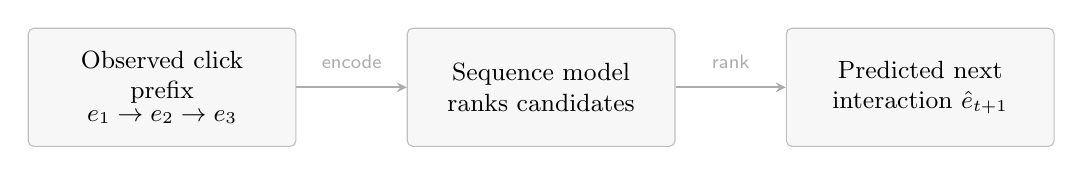
\begin{tikzpicture}[>=stealth, node distance=9mm and 14mm, panel/.style={draw=gray!50, rounded corners=2pt, fill=gray!6, minimum width=34mm, minimum height=15mm, inner sep=3pt, align=center, font=\small}, arrow/.style={->, semithick, draw=gray!65}, label/.style={font=\scriptsize\sffamily, text=gray!65}]
\node[panel] (history) {Observed click\\prefix\\[-1mm] $e_1\rightarrow e_2\rightarrow e_3$};
\node[panel, right=of history] (rank) {Sequence model\\ranks candidates};
\node[panel, right=of rank] (next) {Predicted next\\interaction $\hat e_{t+1}$};
\draw[arrow] (history) -- node[above=3pt, label]{encode} (rank);
\draw[arrow] (rank) -- node[above=3pt, label]{rank} (next);
\end{tikzpicture}
\caption{Redrawn schematic of next-click prediction from an observed click prefix, inspired by the task formulation in Zhou and Li~\cite{zhou2021large}.}
	\label{fig:examplecontacts}
\end{figure}


\begin{figure}[!h]
	\centering
	\includegraphics[width=.6\linewidth]{pages_and_times}
	\caption{User pages and clicks at $t_i$ or different times, showing how the user clicked on elements at different times. For example, the user clicked on the first element at time $t_1$, the second element at time $t_2$, and the third element at time $t_3$ \cite{yang2020measuring}}.
	\label{fig:PagesAndTimes}
\end{figure}

\section{Proposed Model}
% - User Click Behaviors
% - features in the data

The main objective of this study is to \DIFdelbegin \DIFdel{improve user experience by leveraging LSTM and Transformer models. To this end, user interaction data is used to train these models, which are then applied to enhance the UX of a mobile application}\DIFdelend \DIFaddbegin \DIFadd{predict the next user click and examine how the resulting rankings could support UX analysis}\DIFaddend . This section \DIFdelbegin \DIFdel{first describes the }\DIFdelend \DIFaddbegin \DIFadd{describes }\DIFaddend data collection and preprocessing\DIFdelbegin \DIFdel{steps}\DIFdelend , followed by \DIFdelbegin \DIFdel{a brief overview of the LSTM and Transformer architectures for predicting the user's next click }\DIFdelend \DIFaddbegin \DIFadd{the evaluated sequence models }\DIFaddend (see Figure \ref{fig:ModelFlow}). \DIFdelbegin \DIFdel{Finally, the prediction results are utilized to conduct UX evaluations, including }\DIFdelend \DIFaddbegin \DIFadd{The resulting rankings can guide proposed design improvements; the present study does not establish their effects through }\DIFaddend first-click \DIFdelbegin \DIFdel{and usability testing}\DIFdelend \DIFaddbegin \DIFadd{or usability tests}\DIFaddend .

\begin{figure}[!h]
	\centering
	\includegraphics[width=0.8\linewidth]{model_flow}
	\caption{Steps \DIFdelbeginFL \DIFdelFL{of Implementing the Proposed Model }\DIFdelendFL \DIFaddbeginFL \DIFaddFL{for implementing }\DIFaddendFL and \DIFdelbeginFL \DIFdelFL{Enhancing User Experience}\DIFdelendFL \DIFaddbeginFL \DIFaddFL{evaluating the next-click prediction models.}\DIFaddendFL }
	\label{fig:ModelFlow}
\end{figure}


Each page contains several clickable elements (see Figure~\ref{fig:PagesAndClickableElemetnsChart}). When a user clicks on one of these elements, an event is recorded, and the user is redirected to another page with a different set of elements. For example, the \textit{Notifications} page includes a \textit{Back} button that allows the user to return to the previous page. Similarly, the \textit{Home} page features clickable elements such as \textit{Users}, \textit{Market}, \textit{Settings}, and \textit{Notifications}, each of which navigates the user to a different page upon selection.


\begin{figure}[!h]
	\centering
	\includegraphics[width=0.99\linewidth]{pages_and_clickable_elemetns_chart}
	\caption{The number of clickable elements on each page is shown in this chart.  
		For example, Settings page contains 6 clickable elements, while the Notifications page has 1 clickable element.}
	\label{fig:PagesAndClickableElemetnsChart}
\end{figure}
Data was collected via a mobile employee recognition app, using the Metrix\footnote{metrix.ir} platform to label clickable elements. User click sequences were then constructed in preprocessing by concatenating recorded click events from standard users. \DIFaddbegin \DIFadd{The platform recorded an opaque, UUID-formatted MX User Id for each User ID; a consistent numeric replacement code was used for sequence reconstruction and user-disjoint evaluation. Neither identifier was a predictive model input.
}\DIFaddend 

\subsection{Data Preprocessing}
\DIFdelbegin \DIFdel{Initially, the user click events were sorted based on the attributes of `UserID` and `Date and time` to ensure that click events performed by a single user were arranged sequentially in chronological order.
Subsequently, by removing duplicate events and concatenating each click event , more than }\DIFdelend \DIFaddbegin \DIFadd{Click events were ordered by recorded User ID and event time where timestamps were valid. The primary analysis retains consecutive clicks on the same element because repetition may reflect delayed feedback, confusion, accessibility difficulty, or frustration. The analytic dataset contains 46,194 click events in }\DIFaddend 4,\DIFdelbegin \DIFdel{000 click sequences were created. Based on previous research and data analysis tools such as Metrix, Google Analytics, and Firebase}
\DIFdel{, each click sequence was considered in two ways:

}\DIFdelend \DIFaddbegin \DIFadd{223 sequences from 52 recorded User IDs. Session construction and its sensitivity to inactivity thresholds are described below.
}\DIFaddend 

\begin{itemize}
	\item

	This method defines a user's click sequence from the first click until a set expiry time typically two minutes of inactivity. If no click occurs within two minutes, the sequence from the first to the last click is stored (Figure \ref{fig:ExpireTime}).
	\DIFdelbegin \DIFdel{Google Analytics applied this approach for analyzing user behavior on news websites. A four-minute expiry was also tested, resulting in longer but fewer sequences, with minimal impact on overall model results}\DIFdelend \DIFaddbegin \DIFadd{The 120-second and 240-second inactivity cutoffs are evaluated as alternative session-construction settings. They are not assumed to be universal mobile-session durations, and no claim of statistical equivalence is made}\DIFaddend .
	\begin{center}
	\begin{figure}[!h]  \centering \includegraphics[width=0.6\linewidth]{expire_time}  \caption{Illustration of the 120-second inactivity cutoff evaluated for click-sequence construction.} \label{fig:ExpireTime} \end{figure}
		\end{center}

	\item
	Sequence Based on User App Sessions:
	A sequence was defined from the moment the user opened the app until it was closed. In this scenario, the user opened the app, clicked on various parts, and then closed the app, which was recorded as a click sequence.
\end{itemize}
The \DIFdelbegin \DIFdel{2-minute }\DIFdelend \DIFaddbegin \DIFadd{two cutoffs provide a sensitivity check around short mobile interactions rather than a literature-established optimum. In the repeat-inclusive export, 4,185 rows (44,823 clicks) have aligned timestamps for within-row gap analysis. Splitting these rows at gaps greater than 120 }\DIFaddend and \DIFdelbegin \DIFdel{4-minute expiry times were chosen because compact mobile screens lead to faster user interaction and decision-making compared to websites \mbox{%DIFAUXCMD
\cite{nielsen2013mobile}}\hskip0pt%DIFAUXCMD
. This aligns with research showing that average mobile session durations fall between 2 to }\DIFdelend \DIFaddbegin \DIFadd{240 seconds yields 4,306 and }\DIFaddend 4\DIFdelbegin \DIFdel{minutes. Consequently,click sequenceswere recorded using both expiry times,resulting in a four-column dataset (}\DIFdelend \DIFaddbegin \DIFadd{,263 sequences, respectively, without changing the 44,823 observed clicks. Mean sequence lengths are 10.41 and 10.51 clicks, respectively (median 5; 95th percentile 25 in both settings). The corresponding numbers of next-click targets are 40,517 and 40,560. This analysis excludes rows with unusable timestamp alignment; it does not reconstruct the complete original event log or establish that either cutoff is optimal. The event-table fields are illustrated below (}\DIFaddend Figure \ref{fig:dataset1}).

\begin{itemize}
	\item
	Column 1: User ID
	\item
	Column 2: Page
	\item
	Column 3: Clickable Element
	\item
	Column 4: Date and Time
\end{itemize}


\begin{figure}[!h]
\centering
\tiny\sffamily
\sloppy
\hyphenpenalty=10000
\exhyphenpenalty=10000
\renewcommand{\arraystretch}{1.18}
\setlength{\tabcolsep}{3pt}
\arrayrulecolor{gray!35}
\begin{tabular}{>{\centering\arraybackslash}p{0.06\linewidth}|>{\centering\arraybackslash}p{0.40\linewidth}|>{\centering\arraybackslash}p{0.45\linewidth}}
\toprule
\rowcolor{gray!35}\color{black}\textbf{ID} & \color{black}\textbf{Click sequence} & \color{black}\textbf{Time (Gregorian calendar)}\\
\midrule
\rowcolors{2}{gray!8}{white}
4 & marketplace, users, settings & 2023-10-09 00:08:03; 00:08:06; 00:08:09\\ \hline
5 & volunteerEvent, marketplace, dashboard, settings & 2023-10-16 14:38:07; 14:39:53; 14:39:54; 14:39:57\\ \hline
7 & close, volunteerEvent, settings, withdrawRequests, transactions & 2023-10-17 08:34:25; 08:34:47; 08:35:00; 08:35:38; 08:35:40\\ \hline
8 & dashboard, settings, notifications, backNotifications & 2023-10-17 13:56:01; 13:56:53; 13:56:58; 13:57:01\\ \hline
4 & close, users, dashboard, logout, okLogout & 2023-10-17 14:41:03; 14:41:04; 14:41:07; 14:41:09\\ \hline
40 & excellent, normal, submitThermometer, surveysBox, notifications, backNotifications & 2023-10-30 07:36:22; 07:36:22; 07:36:22; 07:36:26; 07:36:33; 07:37:07\\ \hline
5 & close, marketplace, users, dashboard, logout, notifications & 2023-10-31 21:20:54; 21:20:57; 21:20:58; 21:21:08; 21:21:09; 21:21:10\\ \hline
\bottomrule
\end{tabular}
\caption{Examples of user click sequences recorded during app interaction. Dates are shown in the Gregorian calendar; times are retained from the event log.}
\label{fig:dataset1}
\end{figure}

For an event to be considered valid, it must be clickable, visible, and enabled. Some elements may be clickable but inactive, which would still qualify them as verified clickable elements.
\DIFdelbegin \DIFdel{Subsequently, user sequences exhibiting outlier behaviors, such as repeated clicks on the same element, were filtered out. The resulting dataset included more than 35,000 clicks, forming click sequencesof 50 Android users. }\DIFdelend \DIFaddbegin \DIFadd{Repeated clicks are retained in the revised primary analysis. The final analytic dataset contains 46,194 clicks, 4,223 sequences, 52 recorded User IDs, and 93 literal click labels. The User IDs are used for group splitting and are not model inputs.
}\DIFaddend Transitioning from one page to another can occur in several ways:
\begin{itemize}
	\item 
	A new page is opened.
	\item 
	A bottom sheet menu is displayed.
	\item 
	A modal or dialog box is shown.
\end{itemize}



%\begin{figure} \centering \includegraphics[width=1.1\linewidth]{clickable_elements}
%	\caption{Examples of clickable elements, including buttons varients, search field, navigation bar, dialog, and selection controls such as radio button, checkboxe, and toggle\protect\footnotemark}	\label{fig:ClickableElements} \end{figure} \footnotetext{\url{figma.com/community}}

\subsection{Data Modeling}
To model the data, a dataset of user click sequences is obtained after preprocessing. These click sequences are initially performed by a user with a defined expiration time, and the user identifier is recorded in the first column. The second column contains the name of the page where the element was clicked. Subsequently, the user's click sequence across different pages is displayed, with the clicked element in each page documented accordingly. Finally, the date and time of these click sequences are recorded. \DIFdelbegin \DIFdel{This dataset is then used as input to the model}\DIFdelend \DIFaddbegin \DIFadd{The event table supports sequence construction and retrospective diagnostics; the evaluated predictor receives only the observed click-label prefix, not the User ID, page labels, or timestamps}\DIFaddend .

\subsubsection{Sequence Lengths \& Time Spans} 
\DIFdelbegin \DIFdel{The maximum sequence length in the dataset consists of 103 user clicks on various elements, amounting }\DIFdelend \DIFaddbegin \DIFadd{After restoration, sequence length ranges from 1 }\DIFaddend to 1,\DIFdelbegin \DIFdel{159 characters. The minimum sequence length consists of a single user click}\DIFdelend \DIFaddbegin \DIFadd{156 clicks (median 5; mean 10.94). Model context is capped at the last 32 observed clicks, so extremely long repeated-click runs do not increase the input length beyond the prespecified context window}\DIFaddend .

%\subsubsection{User Click Frequencies}
%Click frequencies are used to gain a deeper understanding of user interactions with click sequences. Each application consists of various sections, each offering different features. Identifying the sections where users have the highest number of clicks and determining which sequences attract the most user attention can contribute to improving the user experience in those areas. Additionally, these insights can be utilized to identify issues within the application.


\section{Architectures for Predicting the Next User Click}
%\section{Modeling Click Behaviors}
\label{sec:model}
Following the data collection and preprocessing steps previously outlined, the architectures of two models developed for predicting the next user click are presented in the sections below.

\subsection{Modeling User Click Behavior with LSTM}
\begin{figure}
	\centering
	\includegraphics[width=1\linewidth]{lstm_arc}
	\caption{The architecture of the LSTM model, comprising layers for pages, clickable elements, user click events, tokenization, embedding, and LSTM layers.}
	\label{fig:LstmArc}
\end{figure}

A click event is characterized by attributes such as the page, the element clicked, and the time the click occurred.
The $i$-th event in the click sequence is denoted by $e_i$ and is defined as shown in (Equation \ref{ei}):
\begin{equation}\label{ei}
	e_i=[s_i, c_i, t_i]
\end{equation}

where $s_i$ represents the page in the $i$-th event, $c_i$ denotes the element that was clicked, and $t_i$ indicates the time of the event.
The page \( s_i \) consists of several clickable elements \( c_i \in s_i \), where \( 1 \leq i \leq |s_i| \) and \( |s_i| \) represents the number of clickable elements on the page. Therefore, the click sequence of a user is defined as the set \( e_{i:n} \).
\begin{equation*}\label{ein}
	e_{i:n}=\{(s_1, c_1, t_1), (s_2, c_2, t_2), \ldots, (s_n, c_n, t_n)\}
\end{equation*}

\DIFdelbegin \DIFdel{In this formula, the user click events are extended and written as events from $i$ to $n$, forming }\DIFdelend \DIFaddbegin \DIFadd{The recorded events form }\DIFaddend a click sequence (Figure \ref{fig:LstmArc})\DIFdelbegin \DIFdel{. Subsequently, tokenization is applied to the elements of the user click sequence ${e_{i:n}}$ so that the pages and clickable elements are converted into numerical codes, allowing the model to process them }\DIFdelend \DIFaddbegin \DIFadd{, but the revised predictive models tokenize only the observed clicked-element labels. Page and time remain in the event archive for reconstruction and retrospective analysis; neither is a model feature. The token map is fitted on the training partition and maps an unseen input label to an unknown token }\DIFaddend (Equation \ref{tokenizer4}).
\DIFdelbegin \DIFdel{The role of the tokenizer is to map each element to a unique number, so that tokens can be provided as numerical input to the model.
}\DIFdelend \begin{equation}\label{tokenizer4}
	v_i = \DIFdelbegin \DIFdel{tokenizer}\DIFdelend \DIFaddbegin \operatorname{tokenizer}\DIFaddend (\DIFdelbegin %DIFDELCMD < {%%%
\DIFdel{e_{i:n}}%DIFDELCMD < }%%%
\DIFdelend \DIFaddbegin \DIFadd{c_i}\DIFaddend )
\end{equation}

Then, during embedding, the generated numerical codes are mapped to fixed-dimensional vectors so that these vectors can capture the semantic relationships between words and be used for learning (Equation \ref{embedding4}).
\begin{equation}\label{embedding4}
	embedding(v_i)= v_i \cdot w_e
\end{equation}

In this, $w_e$ is the matrix that holds the embedding weights, where $w_e \in \mathbb{R}^{V \times D}$, and its dimensions depend on the number of words in the vocabulary and the embedding dimensions. $V$ is the number of unique words in the dataset, and $D$ is the dimensionality of the embedding vector, which is a hyperparameter typically set as the number of embedding dimensions.
The first LSTM layer processes the input sequence, models the temporal relationships between the clicks, processes a sequence of vectors $v_i$, and outputs the hidden state $h_t$ (Equation \ref{llstm4}).
\begin{equation}\label{llstm4}
	h_t = l_{lstm} \rightarrow embedding(v_i)
\end{equation}

Where $h_t \in \mathbb{R}^M$ represents an $M$-dimensional space. In the model, this means that the output of each node or unit in this layer will be an $M$-dimensional vector of real numbers. In other words, if $M$ equals 128, each output vector from this layer will have 128 components. For example, in the LSTM layer in the model architecture described, if $M$ is set to 128, each hidden state (denoted as Hidden State) output from this layer will be a vector of real numbers representing the information the model acquires from the data at each step.
The \DIFdelbegin \DIFdel{second LSTM layer processes the output of the first layer and extracts further information from the temporal sequence}\DIFdelend \DIFaddbegin \DIFadd{revised LSTM reference implementation has one 64-unit recurrent layer; the final non-padding hidden state represents the observed prefix}\DIFaddend .
The $Dense$ layer, a fully connected layer, converts the output of the previous layers into a fixed-dimensional vector (Equation \ref{ldense4}).

\begin{equation}\label{ldense4}
	l_{dense} : dense(h_t )
\end{equation}

The $Dropout$ layer randomly disables some neurons during training to prevent overfitting and make the model more generalizable (Equation \ref{ldropout4}).

\begin{equation}\label{ldropout4}
	l_{dropout} : dropout(l_{dense})
\end{equation}

\DIFdelbegin \DIFdel{As a result, the problem of predicting the next user click is defined as (Equation \ref{eincn4}). }\DIFdelend \DIFaddbegin \DIFadd{The prediction task is defined in Equation \ref{eincn4}. At inference time, the model has access only to the observed click labels up to step $n$; it ranks next-click labels from the training vocabulary.
}\DIFaddend 

\DIFdelbegin \begin{displaymath}\DIFdel{%DIFDELCMD < \label{eincn4}%%%

	UNCP\footnote{User Next Click Prediction}(c_{n+1}) =f(s_{n+1}, t_{n+1}, e_{1:n})
}\end{displaymath}%DIFAUXCMD
\DIFdelend \DIFaddbegin \begin{equation}\DIFadd{\label{eincn4}
	\hat{\mathbf p}_{n+1}=f_{\theta}(c_{\max(1,n-L+1):n}),\qquad \hat c_{n+1}=\operatorname*{arg\,max}_{c}\,\hat p_{n+1}(c),\quad L=32
}\end{equation}\DIFaddend 


\DIFdelbegin \DIFdel{Where in this equation, }\DIFdelend \DIFaddbegin \DIFadd{Here $c_{\max(1,n-L+1):n}$ is the last $L=32$ observed click labels (or the shorter available prefix), $f_{\theta}$ returns a probability distribution over next-click labels, and $\hat c_{n+1}$ is its highest-ranked label. The actual next click $c_{n+1}$ is the evaluation target. The destination page }\DIFaddend $s_{n+1}$ \DIFdelbegin \DIFdel{represents the page in the $(n+1)$-th event,
}\DIFdelend \DIFaddbegin \DIFadd{and event time }\DIFaddend $t_{n+1}$ \DIFdelbegin \DIFdel{represents the timestamp of the $(n+1)$-th event,
$e_{1:n}$ represents the click sequence derived from the user's click history as mentioned in previous formulas.
Finally, $c_{n+1}$ represents the User Next Click, which is a function $f$ applied to the aforementioned elements. }\DIFdelend \DIFaddbegin \DIFadd{are known only after that event and are never supplied to $f_{\theta}$. Recorded destination pages are used solely for retrospective page-level diagnostics.
}\DIFaddend 

\subsection{Modeling User Click Behavior with Transformer}
First, a semantic representation of the clicked element in each click event is extracted to better understand the features of the elements and the user's click behavior.
Then, a sequence of click events is modeled to encode the user's click history.
Finally, based on the \DIFdelbegin \DIFdel{encoding of the previous click events, a model is designed to select the element most likely to be clicked from all the active and clickable elements on the current page }\DIFdelend \DIFaddbegin \DIFadd{encoded click history, the reference model ranks next-click labels in the training target vocabulary }\DIFaddend (Figure \ref{fig:TransformerArc}). \DIFaddbegin \DIFadd{It is not given the future destination page or a page-specific candidate mask.
}\DIFaddend 


\begin{figure}
	\centering
	\includegraphics[width=1\linewidth]{transformer_arc}
	\caption{The Transformer architecture, which includes layers for pages, clickable elements, user click events, tokenization, embedding, and Transformer layers such as feed-forward neural networks, normalization, and stack-based encoders.}
	\label{fig:TransformerArc}
\end{figure}


%A click event has features including the page, the element that was clicked, and the time when the click occurred.
%The $i$-th event in the click sequence is denoted by $e_i$ and is defined as (Equation \ref{ei}):
%\begin{equation}\label{ei}
%	e_i=[s_i, c_i, t_i]
%\end{equation}

%Where $s_i$ represents the page in the $i$-th event, $c_i$ is the clickable element that was clicked, and $t_i$ is the time of the event. The page $s_i$ consists of a number of clickable elements $c_i \in s_i$, where $1 \leq i \leq |s_i|$, and $|s_i|$ denotes the number of clickable elements on the page. Therefore, the user's click sequence is defined as the set $e_{i:n}$:

%\begin{equation*}\label{ein}
%	e_{i:n}=\{(s_1, c_1, t_1), (s_2, c_2, t_2), \ldots, (s_n, c_n, t_n)\}
%\end{equation*}


%In this formula, the user's click events are expanded and written as events from $i$ to $n$ to form a click sequence. Next, tokenization is applied to the elements of the user's click sequences ${e_{i:n}}$, converting pages and clickable elements into numerical codes, allowing the model to process them (Equation \ref{tokenizer5}). The role of the tokenizer is to map each element to a unique number, enabling the tokens to be provided as numerical input to the model.

%\begin{equation}\label{tokenizer5}
%	v_i = Tokenizer ({e_{i:n}})
%\end{equation}

\DIFdelbegin \DIFdel{(Equation\ref{ei}) and (\ref{tokenizer4}) from the LSTM model, as explained in the previous section, are similar to those used in the Transformer model }\DIFdelend \DIFaddbegin \DIFadd{The Transformer uses the same observed-click tokenization as the LSTM reference model (Equation \ref{tokenizer4})}\DIFaddend .
In the following, the focus shifts to the embedding layer.

Subsequently, in the embedding step, the generated numerical codes are transformed into fixed-dimensional vectors so that these vectors can capture the semantic relationships between the elements and be used for learning (Equation \ref{embedding5}).

\begin{equation}\label{embedding5}
	\DIFdelbegin \DIFdel{Embed}\DIFdelend \DIFaddbegin \DIFadd{\mathrm{Embed}}\DIFaddend _i = \DIFdelbegin \DIFdel{Embed }\DIFdelend \DIFaddbegin \DIFadd{\mathrm{Embed}}\DIFaddend (\DIFdelbegin \DIFdel{s_i, }\DIFdelend c_i\DIFdelbegin \DIFdel{, t_i}\DIFdelend ) 
\end{equation}

\DIFdelbegin \DIFdel{In the embedding function, each component of the input, including the page, element, and time, is mapped into a vector space using the embedding function. The embeddings of the page , element, and time are then combined to form a single vector}\DIFdelend \DIFaddbegin \DIFadd{Only the observed click label is embedded. The page and timestamp are retained in the event data for retrospective analyses, not concatenated with the model input}\DIFaddend .

\DIFdelbegin \begin{displaymath}
	\DIFdel{Embed'_i = }[\DIFdel{Embed_{s_i}, Embed_{c_i}, Embed_{t_i}}]
\DIFdel{}\end{displaymath}%DIFAUXCMD
%DIFDELCMD < 
%DIFDELCMD < 

%DIFDELCMD < %%%
\DIFdelend In the next step, positional encoding is added to the embedded vector to preserve the order of clicks in the sequence, as the Transformer model inherently does not encode the sequence order (Equation \ref{PositionalEncoding44}).

\begin{equation}\label{PositionalEncoding44}
	Embed_i' = Embed_i + {PositionalEncoding}(i)
\end{equation}

\DIFdelbegin \DIFdel{In the next step, the embedded vectors Embedi \( Embed_i' \) are multiplied by the weight matrices \( W_Q \), \( W_K \), and \( W_V \) to produce the matrices.
$Q$}\DIFdel{, $K$, and $V$}
\DIFdel{In the next step, the embedded vectors Embedi \( Embed_i' \) are multiplied by the weight matrices  \( W_Q \), \( W_K \), and \( W_V \) to produce the matrices. $Q$}
\DIFdel{,
$K$,and $V$}
\DIFdel{To calculate attention , the attention mechanism computes the relationship of each element in the sequence with other elements and assigns an attention score to each element. The SoftmaxSoftmaxSoftmax function normalizes these scores such that their sum equals 1, highlighting the most prominent elements.
The attention scores are then used to weight the ValueValue matrix, producing the final output of the attention mechanism }\DIFdelend \DIFaddbegin \smallskip
\DIFadd{The position-aware embeddings are projected with learned matrices \(W_Q\), \(W_K\), and \(W_V\) to form the query \(Q\), key \(K\), and value \(V\) representations. Scaled dot-product attention applies a row-wise softmax to the query--key scores and uses the resulting weights to combine the values }\DIFaddend (Equation \ref{Attentionmchm4}).

\begin{equation}\label{Attentionmchm4}
	Attention (Q, K, V) = {Softmax}\left(\frac{QK^T}{\sqrt{d_k}}\right) V
\end{equation}
\DIFaddbegin \smallskip
\DIFaddend To compute the dot product between the matrices $Q$ and $K$, the calculation \( QK^T \) is performed first. Here, \( K^T \) is the transpose of the matrix \( K \), where its rows and columns are swapped. This allows the dot product between each Query and each Key to be computed.
For normalization, the values obtained from the dot product \( QK^T \) are divided by \( \sqrt{d_k} \), where \( \sqrt{d_k} \) is the dimensionality of the key. This helps reduce fluctuations in large values and makes the model train more effectively. The reason for using \( \sqrt{d_k} \) is that as the number of dimensions increases, the dot product values become larger, and dividing by \( \sqrt{d_k} \) helps balance these values.
Next, a fully connected neural network $x$ is applied independently to each position in the sequence and normalized to improve the stability of the training process.
In the next step, the remaining connections are added to the network to prevent the vanishing gradient problem. The encoder layers, which include self-attention and fully connected neural networks, are repeated multiple times. This repetition allows the model to learn more complex datasets (Equation \ref{Repeating Encoder Layers}).

% Repeating Encoder Layers
\begin{equation}\label{Repeating Encoder Layers}
	H = {StackedEncoderLayers}(E')
\end{equation}

The repetition of encoder layers is considered one of the key principles in the Transformer model. This means that instead of using a single encoder layer, multiple encoder layers are stacked. This approach allows the model to learn more complex and higher-level features from the data.
It is indicated as the final output after passing through all the encoder layers. These vectors represent higher-level representations of the inputs, which can be utilized for subsequent stages such as computation and predicting the next click.
In the next step, the final hidden state, which is the output of the stacked encoder layers, is passed through a $softmax$ layer to produce a probability distribution, $Prob_{n+1}$, over the potential next clicks (Equation \ref{Calculating Probabilities for the Next Click}).

% Calculating Probabilities for the Next Click
\begin{equation}\label{Calculating Probabilities for the Next Click}
	Prob_{n+1} = {Softmax}(H)
\end{equation}

Finally, the Transformer model is used to predict the probability of which element on the screen, $c_{n+1}$, the user is likely to click on in the $(i+1)$-th step, and to determine the function $f$. The $argmax$ function returns the position or index with the highest probability value (Equation \ref{Predicting the Next Click}).
% Predicting the Next Click
\begin{equation}\label{Predicting the Next Click}
	UNCP{c_{n+1}} = argmax(Prob_{n+1})
\end{equation}


\subsection{\DIFdelbegin \DIFdel{Evaluation of the }\DIFdelend Proposed \DIFdelbegin \DIFdel{Method}\DIFdelend \DIFaddbegin \DIFadd{UNCP Hybrid}\DIFaddend }
\DIFdelbegin \DIFdel{Following the implementation of user next-click prediction modelsusing LSTMs and Transformers, the focus is shifting to leveraging these models to enhance UX. While traditional UX tests are vital for identifying software strengths and weaknesses, they suffer from limitations such as significant time consumption, }\DIFdelend \DIFaddbegin \DIFadd{The proposed User Next Click Predictor (UNCP) preserves the click-sequence input used by the preceding models. A shared 32-dimensional click embedding feeds two parallel branches: a 64-unit GRU for short transition patterns and a two-layer, four-head Transformer for longer contextual dependencies. The final real-token Transformer state is projected to 64 dimensions. A learned sigmoid feature gate mixes the GRU and Transformer states elementwise; layer normalization and dropout precede the global click classifier. Neither future clicks, user identity, page identity, nor timestamps are model inputs. The individual operations are established building blocks; the contribution claimed here is their task-specific gated combination and its leakage-aware evaluation, not universal or first-ever architectural novelty.
}

\paragraph{\DIFadd{UNCP 2 graph-aware extension.}} \DIFadd{UNCP 2 constructs a weighted, undirected click-transition adjacency from encoded training prefixes only, adds self-loops, and applies symmetric degree normalization. One graph propagation step transforms the shared 32-dimensional element embeddings; the resulting graph-aware token vectors feed a 64-unit GRU and a two-layer, four-head Transformer. A masked mean of observed graph token vectors forms a third context state. A learned feature gate combines the GRU state with the average of the Transformer and graph states, followed by layer normalization, dropout, and global classification. The validation and test clicks do not enter graph construction. This is a task-specific combination of established graph, recurrent, and attention operations; the observed advantage is limited to }\DIFaddend the \DIFdelbegin \DIFdel{risk of collecting inaccurate datasets (especially in lab settings), and the inability to test the entire user base.
The persona method, which generalizes results from representative user groups, also fails to reliably produce accurate datasets due to varied user behaviors under different conditions. Furthermore, the periodic nature of UX testing leads to wasted time for researchers. The text concludes by reviewing UX testing methods that have the potential to be executed by models like neural networks}\DIFdelend \DIFaddbegin \DIFadd{reported dataset and split.
}

\paragraph{\DIFadd{UNCP 3 and UNCP 4 exploratory variants.}} \DIFadd{UNCP 3 combines a GRU, Transformer, and a plain-PyTorch structured state-space duality (SSD) recurrence inspired by Mamba-2; it does not use the official optimized Mamba-2 kernel. UNCP 4 combines typed page--element graph attention, a training-only transition graph, a GRU, an adaptive fusion gate, and candidate masking. Its mask uses the last observed click's inventory page as a proxy for the current page, augmented with training-observed successors; 33 of 93 click-label strings lack an exact inventory match and use an unrestricted fallback. Neither variant improved on UNCP 2 in the held-out-user experiment, so they are retained as transparent exploratory comparisons rather than selected as the final predictor}\DIFaddend .

\DIFaddbegin \paragraph{\DIFadd{UNCP 5 adaptive transition fusion.}} \DIFadd{UNCP 5 combines the trained UNCP 2 probability vector with a smoothed back-off transition distribution over the last one to four observed clicks. Transition counts and the global smoothing prior use training examples only. The transition weight is a sigmoid function of log transition support and the difference between the two predictive entropies; the final probability vector is their convex combination. We selected the three gate coefficients from a fixed grid of 76 rules by mean validation Top-3 across seeds 11, 23, and 37, breaking ties by validation Top-1 and negative log-likelihood. Only after freezing that choice did we evaluate the held-out users. Thus UNCP 5 is an adaptive probability-level ensemble, not a newly trained end-to-end neural architecture. No future page, timestamp, click, or test label is used to build the transition model or select its gate.
}

\paragraph{\DIFadd{UNCP 6 repeat-aware dual-scale model.}} \DIFadd{One GRU encodes the complete observed click prefix. A second GRU encodes consecutive runs after repeated labels are compressed, with each run length embedded as a feature. A learned gate combines the two states. The next-click distribution factorizes into a repeat-versus-switch probability and a classifier over elements conditional on switching; the repeat option is the last observed label. No future click is used in run construction. Three fixed-seed fits on the same user-disjoint split reach 84.08\% mean Top-3, below UNCP 5's 85.09\%. On the 1,541 repeated-click targets, their Top-3 values are 94.09\% and 94.07\%, respectively; on 9,292 switch targets they are 82.42\% and 83.60\%. This diagnostic prevents a gain on repeats from being mistaken for better prediction of changed actions.
}

\subsection{\DIFadd{Potential Decision Support for UX Analysis}}
\DIFadd{The evaluated models rank likely next clicks from previously observed click sequences. These rankings may help UX researchers identify recurrent transitions, unexpected paths, and interface elements that merit inspection. They do not measure user intent, task success, cognitive load, satisfaction, or usability, and they are not equivalent to conventional UX testing. Whether they reduce evaluation time or effort must be established in a prospective comparison with an existing UX workflow.
}

\DIFaddend \begin{itemize} \item \DIFdelbegin \textbf{\DIFdel{Usability Testing with Neural Network Architectures to Improve User Experience:}}
	%DIFAUXCMD
\DIFdel{To perform usability testing with LSTM and Transformer architectures, various user workflows and scenarios that users have gone through are examined as user clicksequences to determine which scenarios were completed correctly and which ones were incomplete.
By predicting the user's next click , the subsequent steps of these scenarios can also be identified. These models output the final result from multiple different scenarios by understanding the history of the user's previous clicks. A sequence of various program scenarios is provided as input to the model,and the next user click prediction is displayed in the output (Figure \ref{fig:PredictionNextUserClick} )}\DIFdelend \DIFaddbegin \textbf{\DIFadd{Supporting inspection of interaction flows:}}
	\DIFadd{Observed click sequences and predicted next-click rankings can be used to flag common or unexpected paths for later review. The model cannot determine from clickstream data alone whether a task was completed correctly or why a user selected an element. Figure \ref{fig:PredictionNextUserClick} illustrates the prediction task rather than a completed usability test}\DIFaddend . \end{itemize}

\begin{figure}[!h]
	\centering
	\includegraphics[width=0.8\linewidth]{prediction_next_user_click}
	\caption{\DIFdelbeginFL \DIFdelFL{Usability testing and next click }\DIFdelendFL \DIFaddbeginFL \DIFaddFL{Next-click }\DIFaddendFL prediction \DIFdelbeginFL \DIFdelFL{involve tracking sequential user clicks across pages until }\DIFdelendFL \DIFaddbeginFL \DIFaddFL{uses }\DIFaddendFL an \DIFdelbeginFL \DIFdelFL{expiration date is met }\DIFdelendFL \DIFaddbeginFL \DIFaddFL{observed click prefix to rank possible subsequent interactions }\DIFaddendFL \cite{zhou2021large}.}
	\label{fig:PredictionNextUserClick}
\end{figure}

\begin{itemize} \item \textbf{\DIFdelbegin \DIFdel{First Click Testing with neural network architectures to improve user experience}\DIFdelend \DIFaddbegin \DIFadd{Supporting first-click analysis}\DIFaddend :} \DIFdelbegin \DIFdel{For conducting usability testing with LSTM and Transformer architectures, the user's first click in the sequences is filtered to understand the user's initial reaction when first interacting with the application. This is important for identifying elements that are frequently used during }\DIFdelend \DIFaddbegin \DIFadd{Initial-click frequencies may indicate which elements attract interaction and can help select screens for a formal first-click study. They do not establish whether a first click is correct for a task or explain }\DIFaddend the user's \DIFdelbegin \DIFdel{first encounter }\DIFdelend \DIFaddbegin \DIFadd{intent }\DIFaddend \cite{falkowska2022replication}.
	\item \textbf{\DIFdelbegin \DIFdel{Card sorting test with neural network architectures to improve user experience}\DIFdelend \DIFaddbegin \DIFadd{Supporting information-architecture review}\DIFaddend :}
	\DIFdelbegin \DIFdel{For conducting card sorting with LSTM and Transformer architectures, it is sufficient to predict all clickable elements on the page and then sort them in descending order. The results are useful for understanding the visual hierarchy within the application. 
	Analyzing the data from this method helps UX designers discover user patterns when interacting with pages, thereby optimizing the software structure to be more user-centered }\DIFdelend \DIFaddbegin \DIFadd{Ranked click patterns may suggest changes to element prominence and navigation. They are not a substitute for card sorting, which directly examines users' conceptual groupings and labels }\DIFaddend \cite{nawaz2012comparison}.

\end{itemize}


\subsection{Evaluation Metrics}
Evaluation metrics are used to assess the performance of different models. These metrics help determine how well the models have performed and whether they can make accurate predictions. Several metrics are calculated to evaluate the quality of predictions for each method, which are listed below.

\DIFaddbegin \DIFadd{The primary test holds out complete User IDs. We assigned all sequences of each recorded User ID to exactly one of the training, validation, or test partitions before creating overlapping click-prefix examples. The 46,194 figure counts click events, whereas the split counts below are supervised next-click targets. A sequence of length $L$ produces $L-1$ targets; therefore, 46,194 events across 4,223 sequences produce $46{,}194-4{,}223=41{,}971$ targets. The fixed split contains 32, 9, and 11 User IDs, respectively ($32+9+11=52$), and yields 25,399 training, 5,739 validation, and 10,833 test targets ($25{,}399+5{,}739+10{,}833=41{,}971$). Automated protocol checks confirmed that no User ID or source sequence occurs in more than one partition. The vocabulary, popularity counts, transition frequencies, and smoothing priors are derived only from training data. Validation data select checkpoints and the UNCP 5 fusion rule; the test partition is evaluated after those choices are fixed. These checks and the split manifest accompany the executable experiment files.
\DIFadd{For the ``Uniform expected'' baseline, each test target is assigned equal probability over the evaluation candidate vocabulary. If the candidate set has size $K$, sampling uniformly without replacement gives an expected Top-1 accuracy of $1/K$ and an expected Top-3 accuracy of $\min(3,K)/K$. The reported 1.10\% Top-1 and 3.30\% Top-3 values therefore correspond to the 93-label global candidate vocabulary ($1/93$ and $3/93$, rounded to two decimals). This analytical expectation is not estimated from random draws. Page-conditioned uniform diagnostics are reported separately because their candidate sets and page availability are distinct from the global-label task.}
}

\DIFaddend \subsubsection{Top-K Accuracy:}
In this metric, the model's accuracy is calculated based on the number of times the target element appears among the top K predictions of the model. For example, to compute `Top-1 Accuracy` and `Top-3 Accuracy,` the number of times the target element appears within the first and third predictions of the model, respectively, is reported. The higher the value of this metric, the better, as it indicates that the model has performed better in identifying the target elements.

\subsubsection{Absolute Ranking Position:}
This metric refers to the ranking position of the target element among all predictions. The lower the value of this metric, the better, as it indicates that the target element is placed in a higher position among the predictions.

\subsubsection{Relative Ranking Position:}

A relative ranking metric \DIFdelbegin \DIFdel{, calculated as the absolute }\DIFdelend \DIFaddbegin \DIFadd{divides the target's absolute rank by the number of candidate elements. Lower values indicate a better }\DIFaddend rank\DIFdelbegin \DIFdel{divided by the total elements(value in $[0, 1)$, indicates better performance when lower}\DIFdelend . This metric complements \DIFdelbegin \DIFdel{$Top-K Accuracy$ by focusing on the positional importance of the targetelement }\DIFdelend \DIFaddbegin \DIFadd{Top-K accuracy by describing the target's position }\DIFaddend relative to the \DIFdelbegin \DIFdel{page }\DIFdelend \DIFaddbegin \DIFadd{candidate-set }\DIFaddend size, as \DIFdelbegin \DIFdel{described }\DIFdelend \DIFaddbegin \DIFadd{discussed }\DIFaddend in \cite{zhou2021large}.

\DIFdelbegin \DIFdel{Data Preparation.}
\DIFdel{To predict the next user click using the data, it is divided into two sets: training and testing. This division is made with 80\%allocated for training and 20\% for testing.
The purpose of this division is to use the training data to train the model and }\DIFdelend \DIFaddbegin \DIFadd{In addition to micro Top-1 and Top-3 accuracy, we report macro averages across held-out User IDs and target labels, results by recorded page and by training-label frequency group, and candidate-set diagnostics. Neural models are trained with seeds 11, 23, and 37; tables show the mean and sample standard deviation across these runs. For selected paired comparisons, we resample held-out Users as clusters to obtain exploratory confidence intervals and use paired User-level tests with multiplicity correction. Page labels recorded with the eventual click are used only for retrospective diagnostics, not as inference-time inputs. Within-row 120- and 240-second gap refinements and a collapsed-repeat variant assess preprocessing sensitivity. On the same grouped-User-ID assignment, }\DIFaddend the \DIFdelbegin \DIFdel{testing data to evaluate the model. Given that 4216 click sequences are provided as }\DIFdelend \DIFaddbegin \DIFadd{first-order Markov Top-3 scores for the two gap settings are 65.07\% and 65.10\%, and }\DIFaddend the \DIFdelbegin \DIFdel{dataset for the model, }\DIFdelend \DIFaddbegin \DIFadd{fourth-order back-off Markov scores are 79.39\% }\DIFaddend and \DIFdelbegin \DIFdel{20\%of the data is set aside for testing, the number of test data points is determined to be 843. These test sequences are then used for prediction. }\DIFdelend \DIFaddbegin \DIFadd{79.48\%, respectively (10,798 and 10,804 test targets). These are descriptive comparisons on changed target sets, not statistical evidence of equivalence or causal threshold effects. The LSTM and Transformer scores reported for the earlier, smaller aligned-event reconstruction are not attributed to this repeat-inclusive sensitivity analysis.
}\DIFaddend 

\DIFaddbegin \subsection{\DIFadd{Data Preparation}}
\DIFadd{The original implementation expanded 4,216 recorded sequences into overlapping prefix--target examples and then randomly split those examples. A reconstruction showed that 6,061 of 6,215 historical test examples shared their source sequence with training, and all 52 recorded User IDs occurred in both partitions. The historical 88.91\% LSTM Top-3 result is therefore retained only as context and is not used as evidence of unseen-user generalization. After repeated-click restoration, the revised dataset contains 46,194 click events in 4,223 sequences. Because the first event of each sequence supplies context but has no preceding click from which to form a target, these data produce $46{,}194-4{,}223=41{,}971$ next-click targets.
}

\DIFadd{For the revised primary evaluation, complete User IDs are assigned before prefix generation: 32 IDs for training, 9 for validation, and 11 for testing, yielding 25,399/5,739/10,833 next-click targets. The User ID counts sum to 52 and the target counts sum to 41,971, exactly matching the totals above. Vocabulary and frequency statistics are fitted on training data only, validation loss selects checkpoints, and targets unseen during training are scored incorrect. Neural models are run with seeds 11, 23, and 37. A secondary chronological analysis uses only rows with aligned, valid timestamps; because its cohort differs, it is reported separately rather than interpreted as an improvement over the user-disjoint test.
}


\DIFaddend \subsection{Quantitative Evaluation Results}
\DIFaddbegin \DIFadd{The same held-out users and 10,833 prediction targets are used for every method in Table~\ref{tab:compact-results}. Fitted neural models and the adaptive ensemble report the mean of seeds 11, 23, and 37. In descending Top-3 order, the proposed variants are UNCP 5 (85.09\%), UNCP 6 (84.08\%), UNCP 2 (83.58\%), UNCP (82.30\%), UNCP 3 (81.40\%), and UNCP 4 (81.08\%). The table is ordered by increasing Top-3 accuracy so that the highest result appears last. UNCP 5's paired gain over UNCP 2 is 1.51 percentage points, with an exploratory user-cluster bootstrap interval of 1.03--1.77 points over 11 held-out users. Gate coefficients were selected only on validation users.
}

\newcommand{\modeldetail}[1]{{\footnotesize\color{green!35!black}(#1)}}
\newcommand{\score}[2]{#1\,{\color{black!55}\scriptscriptstyle\pm\,#2}}
\newcommand{\uncpbase}{UNCP \modeldetail{GRU--Transformer fusion}}
\newcommand{\uncptwo}{UNCP 2 \modeldetail{transition-graph-aware GRU--Transformer}}
\newcommand{\uncpthree}{UNCP 3 \modeldetail{GRU, Transformer, Mamba-2-inspired SSD}}
\newcommand{\uncpfour}{UNCP 4 \modeldetail{typed graph attention, GRU, transition graph, candidate masking, adaptive fusion}}
\newcommand{\uncpfive}{\textbf{UNCP 5} \modeldetail{UNCP 2, transition model, adaptive fusion}}
\newcommand{\uncpsix}{UNCP 6 \modeldetail{dual GRU streams, run lengths, repeat/switch head}}

\begin{table}[!htbp]
\centering
\caption{\DIFaddFL{Held-out account comparison, sorted by increasing Top-3 accuracy (percent; fitted models report mean $\pm$ sample SD over three seeds).}}
\label{tab:compact-results}
\small
\begin{tabular}{@{}p{.53\linewidth}rr@{}}
\toprule
\DIFaddFL{Model }& \DIFaddFL{Top-1 }& \DIFaddFL{Top-3 }\\
\midrule
\DIFaddFL{Uniform expected }& \DIFaddFL{1.10 }& \DIFaddFL{3.30 }\\
\DIFaddFL{Global popularity }& \DIFaddFL{5.16 }& \DIFaddFL{22.37 }\\
\DIFaddFL{Logistic regression }& \DIFaddFL{$\score{44.24}{0.61}$ }& \DIFaddFL{$\score{71.58}{0.33}$ }\\
\DIFaddFL{Transformer }& \DIFaddFL{$\score{44.46}{0.52}$ }& \DIFaddFL{$\score{71.92}{0.36}$ }\\
\DIFaddFL{RNN }& \DIFaddFL{$\score{50.22}{0.26}$ }& \DIFaddFL{$\score{75.10}{0.48}$ }\\
\DIFaddFL{LSTM }& \DIFaddFL{$\score{54.52}{0.06}$ }& \DIFaddFL{$\score{78.00}{0.55}$ }\\
\DIFaddFL{GRU }& \DIFaddFL{$\score{55.97}{0.62}$ }& \DIFaddFL{$\score{78.88}{0.40}$ }\\
\DIFaddFL{Markov-4 }& \DIFaddFL{60.27 }& \DIFaddFL{79.91 }\\
\uncpfour & \DIFaddFL{$\score{59.84}{1.40}$ }& \DIFaddFL{$\score{81.08}{0.88}$ }\\
\uncpthree & \DIFaddFL{$\score{61.12}{2.29}$ }& \DIFaddFL{$\score{81.40}{0.82}$ }\\
\uncpbase & \DIFaddFL{$\score{62.72}{0.95}$ }& \DIFaddFL{$\score{82.30}{0.52}$ }\\
\uncptwo & \DIFaddFL{$\score{64.62}{1.10}$ }& \DIFaddFL{$\score{83.58}{0.04}$ }\\
\uncpsix & \DIFaddFL{$\score{66.60}{0.51}$ }& \DIFaddFL{$\score{84.08}{0.22}$ }\\
\uncpfive & \DIFaddFL{$\mathbf{\score{66.71}{0.84}}$ }& \DIFaddFL{$\mathbf{\score{85.09}{0.20}}$ }\\
\bottomrule
\end{tabular}
\end{table}

\begin{figure}[!htbp]
\centering
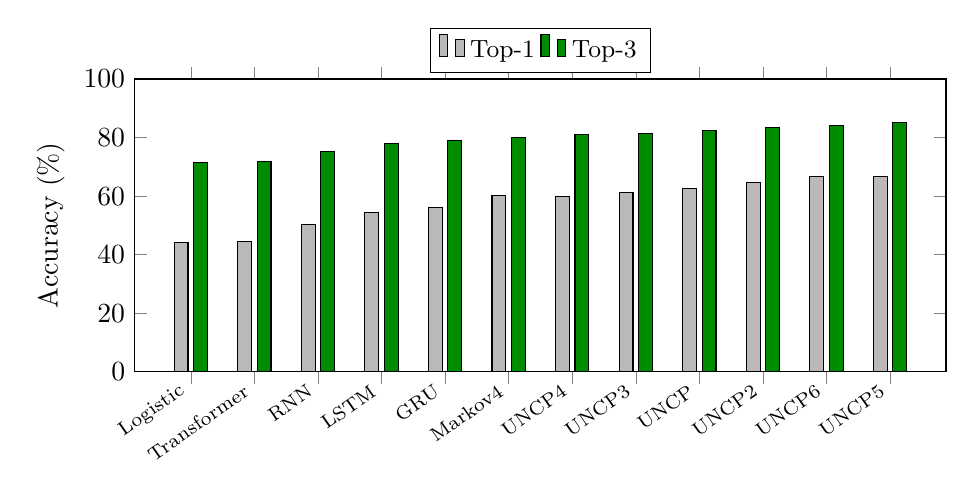
\begin{tikzpicture}
\begin{axis}[ybar,width=.98\linewidth,height=5.3cm,ymin=0,ymax=100,
symbolic x coords={Logistic,Transformer,RNN,LSTM,GRU,Markov4,UNCP4,UNCP3,UNCP,UNCP2,UNCP6,UNCP5},
xtick=data,x tick label style={rotate=35,anchor=east,font=\scriptsize},
ytick={0,20,40,60,80,100},ylabel={Accuracy (\%)},
bar width=5pt,legend style={at={(.5,1.02)},anchor=south,legend columns=2,font=\small},
enlarge x limits=.08]
\addplot[fill=gray!55] coordinates {(Logistic,44.24)(Transformer,44.46)(RNN,50.22)(LSTM,54.52)(GRU,55.97)(Markov4,60.27)(UNCP4,59.84)(UNCP3,61.12)(UNCP,62.72)(UNCP2,64.62)(UNCP6,66.60)(UNCP5,66.71)};
\addplot[fill=green!55!black] coordinates {(Logistic,71.58)(Transformer,71.92)(RNN,75.10)(LSTM,78.00)(GRU,78.88)(Markov4,79.91)(UNCP4,81.08)(UNCP3,81.40)(UNCP,82.30)(UNCP2,83.58)(UNCP6,84.08)(UNCP5,85.09)};
\legend{Top-1,Top-3}
\end{axis}
\end{tikzpicture}
\caption{\DIFaddFL{Updated Top-1 and Top-3 comparison on the user-disjoint test set. Values are generated directly from the verified result files.}}
\label{fig:updated-accuracy}
\end{figure}

\DIFadd{Table~\ref{tab:protocol-results} provides the second and final result table. The temporal subset is a separate robustness analysis with a different eligible cohort, not a directly comparable improvement over the user-disjoint split. UNCP 2--6 have not been evaluated on that subset; their temporal cells are intentionally left unreported. The figure retains the visual comparison used in the original article while replacing the historical contaminated-split scores with the new protocol results.
}

\begin{table}[!htbp]
\centering
\caption{\DIFaddFL{Top-3 accuracy under two leakage-aware protocols, ordered by increasing held-out-user accuracy (percent). A dash denotes an unrun temporal experiment.}}
\label{tab:protocol-results}
\small
\begin{tabular}{@{}p{.53\linewidth}rr@{}}
\toprule
\DIFaddFL{Model }& \DIFaddFL{Held-out users }& \DIFaddFL{Temporal subset }\\
\midrule
\DIFaddFL{Transformer }& \DIFaddFL{71.92 }& \DIFaddFL{73.59 }\\
\DIFaddFL{RNN }& \DIFaddFL{75.10 }& \DIFaddFL{--- }\\
\DIFaddFL{LSTM }& \DIFaddFL{78.00 }& \DIFaddFL{83.84 }\\
\DIFaddFL{GRU }& \DIFaddFL{78.88 }& \DIFaddFL{84.74 }\\
\DIFaddFL{Markov-4 }& \DIFaddFL{79.91 }& \DIFaddFL{88.15 }\\
\uncpfour & \DIFaddFL{81.08 }& \DIFaddFL{--- }\\
\uncpthree & \DIFaddFL{81.40 }& \DIFaddFL{--- }\\
\uncpbase & \DIFaddFL{82.30 }& \textbf{\DIFaddFL{89.95}} \\
\uncptwo & \DIFaddFL{83.58 }& \DIFaddFL{--- }\\
\uncpsix & \DIFaddFL{84.08 }& \DIFaddFL{--- }\\
\uncpfive & \textbf{\DIFaddFL{85.09}} & \DIFaddFL{--- }\\
\bottomrule
\end{tabular}
\end{table}

\begin{figure}[!htbp]
\centering
\begin{subfigure}{.49\linewidth}
\centering
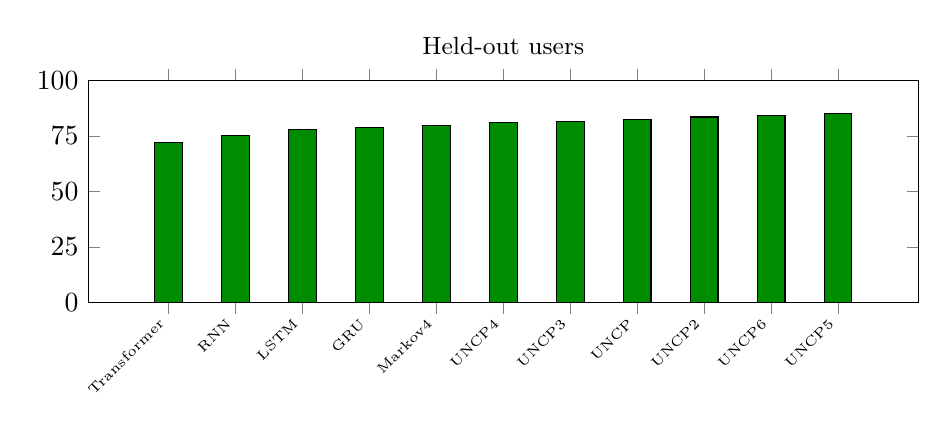
\begin{tikzpicture}
\begin{axis}[ybar,width=\linewidth,height=4.4cm,ymin=0,ymax=100,
symbolic x coords={Transformer,RNN,LSTM,GRU,Markov4,UNCP4,UNCP3,UNCP,UNCP2,UNCP6,UNCP5},xtick=data,
x tick label style={rotate=45,anchor=east,font=\tiny},ytick={0,25,50,75,100},
title={Held-out users},title style={font=\small},bar width=10pt,enlarge x limits=.12]
\addplot[fill=green!55!black] coordinates {(Transformer,71.92)(RNN,75.10)(LSTM,78.00)(GRU,78.88)(Markov4,79.91)(UNCP4,81.08)(UNCP3,81.40)(UNCP,82.30)(UNCP2,83.58)(UNCP6,84.08)(UNCP5,85.09)};
\end{axis}
\end{tikzpicture}
\end{subfigure}
\begin{subfigure}{.49\linewidth}
\centering
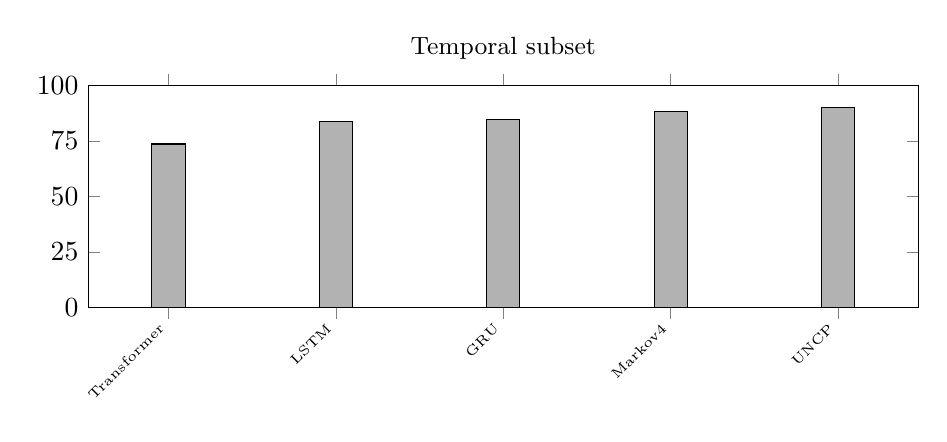
\begin{tikzpicture}
\begin{axis}[ybar,width=\linewidth,height=4.4cm,ymin=0,ymax=100,
symbolic x coords={Transformer,LSTM,GRU,Markov4,UNCP},xtick=data,
x tick label style={rotate=45,anchor=east,font=\tiny},ytick={0,25,50,75,100},
title={Temporal subset},title style={font=\small},bar width=12pt,enlarge x limits=.12]
\addplot[fill=gray!60] coordinates {(Transformer,73.59)(LSTM,83.84)(GRU,84.74)(Markov4,88.15)(UNCP,89.95)};
\end{axis}
\end{tikzpicture}
\end{subfigure}
\caption{\DIFaddFL{Top-3 accuracy for selected models under the held-out-user and qualified temporal protocols.}}
\label{fig:updated-protocols}
\end{figure}

\DIFadd{Top-1 requires the observed next click to be the highest-ranked prediction, whereas Top-3 counts success when it appears among the three highest scores. Both are reported because Top-3 is useful for ranking candidate interactions, but it must be interpreted alongside transparent baselines and the candidate space. Numerical comparisons with other publications are not used to claim superiority because their datasets, interfaces, labels, and split procedures differ.
}

\iffalse
\DIFaddend After evaluating and implementing Transformer neural network models, sequence modeling, Recurrent Neural Networks, and LSTM in the learning periods, the following results were achieved using the evaluation metrics: Top-1 accuracy (Figure \ref{fig:Models Top1 Accuracy}), Top-3 accuracy (Figure \ref{fig:Models Top3 Accuracy}), Absolute Ranking Position (Figure \ref{fig:Absolute Ranking Position}), and Relative Ranking Position (Figure \ref{fig:Relative Ranking Position}). It should be noted that, in addition to the aforementioned models, another model called `Sequence Modeling` was also utilized, and the results of all these models, along with the evaluation metrics `Top-1 Accuracy` and `Top-3 Accuracy,` are presented.
By comparing the results with those from other studies, the LSTM and Transformer models from Zhou and Li were also included. The results indicate that a relatively higher accuracy for predicting the next user click was achieved compared to the approaches and architectures used in previous research. However, the differences in results arise from the model provided, the dataset, and the methods and approaches used, distinguishing it from other studies.
For Top-3 accuracy, the sequence modeling achieved an accuracy of 84\%, while the LSTM model achieved an accuracy of nearly 89\%. This approximately 5\% difference suggests that if the model used Top-3 accuracy instead of Top-1 accuracy, better results could be obtained.

\subsubsection{Top-1 vs. Top-3 Accuracy Discrepancy}
Top-1 accuracy in User Next Click Prediction requires an exact match with the user\DIFdelbegin \DIFdel{?}\DIFdelend \DIFaddbegin \DIFadd{'}\DIFaddend s click, while Top-3 accuracy includes correct actions within the top three predictions. This distinction is important in contexts with multiple relevant options, as Top-3 better reflects the model?s ability to identify user intentions. Reporting both metrics offers a fuller evaluation of the model?s real-world performance.


\subsubsection{Model Accuracy and Practical Implications}
Our model achieved a Top-3 prediction accuracy of 0.88, which is substantially higher than those reported in previous studies. For instance, Zhou and Li \cite{zhou2021large} report a Top-3 accuracy of 0.71 for their proposed model and 0.64 for a Transformer-based model. The baseline Logistic Regression model in the same study reached only 0.53.  This performance demonstrates the superior predictive power of our approach.

In practical terms, such high accuracy offers considerable benefits. For example, across 10 distinct pages with multiple clickable elements, our model is able to correctly predict the next user click within the top three predicted options in approximately 9 out of 10 cases. This capability allows researchers to automate common UX testing procedures such as First Click Tests and Usability Evaluations based solely on clickstream data.

Consequently, UX designers can better understand user behavior and make informed improvements to enhance the usability and effectiveness of their interfaces.

\begin{figure}[htbp]
	\centering
	\begin{subfigure}[b]{0.48\textwidth}
		\centering
		\includegraphics[width=\textwidth]{models_top1_accuracy}
		\caption{Top-1 accuracy }
\label{fig:models-top1-accuracy}
	\end{subfigure}
	\hfill
	\begin{subfigure}[b]{0.48\textwidth}
		\centering
		\includegraphics[width=\textwidth]{models_top3_accuracy}
		\caption{Top-3 accuracy}
\label{fig:models-top3-accuracy}
	\end{subfigure}
	\caption{Comparison of models with Top-1 and Top-3 accuracy evaluation metric}
	\label{fig:twofigures}
\end{figure}



%\begin{figure}
%	\centering
%	\includegraphics[width=1\linewidth]{models_top1_accuracy}
%	\caption{Comparison of models with Top-1 accuracy evaluation metric}
%	\label{fig:Models Top1 Accuracy}
%\end{figure}
%
%\begin{figure}
%	\centering
%	\includegraphics[width=1\linewidth]{models_top3_accuracy}
%	\caption{Comparison of models with Top-3 accuracy evaluation metric}
%	\label{fig:Models Top3 Accuracy}
%\end{figure}
\begin{figure}[htbp]
	\centering
	\begin{subfigure}[b]{0.48\textwidth}
		\centering
		\includegraphics[width=\textwidth]{absolute_ranking_position}
		\caption{Absolute Ranking Position}
\label{fig:absolute-ranking-position}
	\end{subfigure}
	\hfill
	\begin{subfigure}[b]{0.48\textwidth}
		\centering
		\includegraphics[width=\textwidth]{relative_ranking_position}
		\caption{Relative Ranking Position}
\label{fig:relative-ranking-position}
	\end{subfigure}
	\caption{Comparison of models with Absolute and  Relative Ranking Position evaluation metric}
\label{fig:ranking-comparison}
\end{figure}

%\begin{figure}
%	\centering
%	\includegraphics[width=1\linewidth]{absolute_ranking_position}
%	\caption{Relative Ranking Position}
%	\label{fig:Absolute Ranking Position}
%\end{figure}
%
%\begin{figure}
%	\centering
%	\includegraphics[width=1\linewidth]{relative_ranking_position}
%	\caption{Comparison of models with Relative Ranking Position evaluation metric}
%	\label{fig:Relative Ranking Position}
%\end{figure}

\DIFaddbegin \fi
\DIFaddend \subsection{User Interface Elements}
The dataset contains a variety of user interface elements, including a total of 65 clickable items distributed across 15 pages. These elements include buttons, search fields, text fields, icons, modals, sorting options, filters, and tags. The results, which show the frequency of clicks on each element across the interface pages, indicate that the most frequently clicked items were found in the \textit{Organizational Thermometer} and \textit{Employee Status} sections under Human Resources. In contrast, the least clicked elements were located in the \textit{Wallet} and \textit{Sorting} sections.

\DIFaddbegin \DIFadd{The supplied analytic export contains 93 distinct click-label strings and 19 recorded page strings; these strings are not a verified inventory of unique widgets or screens. The earlier 65-element/15-page design description is therefore retained as application context pending reconciliation with the source interface inventory. Page-based analyses are retrospective and no future destination-page label is supplied to the prediction models.
}



\DIFaddend %\begin{figure}
%	\centering
%	\includegraphics[width=0.4\linewidth]{google_calendarapp}
%	\caption{An example of clickable elements in the Google Calendar mobile app.}
%	\label{fig:googlecalendarapp}
%\end{figure}


\subsection{\DIFdelbegin \DIFdel{User Experience Improvement Evaluation}\DIFdelend \DIFaddbegin \DIFadd{Proposed UX Improvements}\DIFaddend }
\DIFdelbegin \DIFdel{To evaluate the improvement of the user experience, the results obtained from predicting the next user click and user experience tests were used to enhance various sections of the app, including the }\DIFdelend \DIFaddbegin \DIFadd{The predicted rankings and observed click patterns motivated possible changes to the }\DIFaddend `Settings,` `Home,` `Marketplace,` and `Users` pages. \DIFdelbegin \DIFdel{On the `Settings ` page, the list of features available was sorted by priority and usage frequency, so that users would see and interact with the most frequently used elements at the top of the list. This was also applied to the bottom menu of the `Home ` page, which contains several iconssuch as `Home, ` `Marketplace, ` `Users,` and `Settings,` to ensure that users were faced with the elements they had interacted with the most. On the `Marketplace` page, items or services with the highest sales were sorted, and the option to sort by most purchased items was added to make them more accessible to users.
On the `Users` page, the option to show users with the highest coin balance was implemented.

}\DIFdelend \DIFaddbegin \DIFadd{These included prioritizing frequently used Settings items, reconsidering the order of Home navigation icons, adding purchase-based sorting on Marketplace, and providing a coin-balance ordering option on Users. These proposals illustrate how prediction may inform design review; the study did not measure whether they improved usability or reduced evaluation effort.
}\DIFaddend 

The \DIFdelbegin \DIFdel{first-click test showed that users frequently clicked }\DIFdelend \DIFaddbegin \DIFadd{archived clickstream contained frequent clicks on }\DIFaddend the `Close` icon in the \DIFdelbegin \DIFdel{status entry menu in }\DIFdelend \DIFaddbegin \DIFadd{status-entry menu of }\DIFaddend the organizational thermometer\DIFdelbegin \DIFdel{, indicating that they did not need to repeatedly interact with this menu in a way that could become annoying. For example, users can click the }\DIFdelend \DIFaddbegin \DIFadd{. This pattern suggests that repeated presentation of the menu merits investigation. Possible design responses include a }\DIFaddend `Do not show again` option, \DIFdelbegin \DIFdel{and they will not encounter this menu upon each app launch. Another solution implemented was that by selecting this option, the section would not appear for a day, or the system administrator could customize the display time of this modal. For example, the modal would not be shown again until after a certain period since the user's last entry, so it wouldn't be bothersome}\DIFdelend \DIFaddbegin \DIFadd{a temporary dismissal period, or administrator-configurable display timing. The click log alone does not establish that the menu caused annoyance or that these changes would improve the experience}\DIFaddend .

\DIFdelbegin \DIFdel{Additionally, on the toolbar at the top of the app, users have the option to register their status }\DIFdelend \DIFaddbegin \DIFadd{The toolbar also allows status registration }\DIFaddend at any time. This \DIFdelbegin \DIFdel{demonstrates that users might even exit the app with a single click and not return, which is why in marketing and increasing customer loyalty, the app needs to be designed in a way that captures the user 's attention and meets their needs as quickly as possible during their first interaction}\DIFdelend \DIFaddbegin \DIFadd{observation may inform a review of early-session interaction and feature visibility, but the available data do not measure attention, loyalty, satisfaction, or the reason a user leaves the application}\DIFaddend .

\DIFdelbegin \DIFdel{Finally, after retesting with some users and evaluating them, it was determined that the scenarios and user interaction flows with the app had improved, the length of the sequences had decreased, and the user flows had become less complex compared to before. }\DIFdelend \DIFaddbegin \DIFadd{These proposed improvements are informed by observed click patterns. Recorded outcomes from the stated retest are unavailable; therefore, this study does not claim that task success, satisfaction, sequence length, or usability improved. A prospective controlled user study is required to evaluate those outcomes.
}\DIFaddend 

\DIFaddbegin \DIFadd{Future evaluation should test the proposed Settings ordering, Home navigation, Marketplace sorting, Users ordering, and thermometer dismissal options with comparable tasks on the existing and redesigned interfaces. A controlled study can measure task success, completion time, navigation errors, repeated or backtracking clicks, and validated usability and satisfaction scores. First-click tasks and card-sorting exercises should be conducted as distinct user studies where relevant. This would determine which proposed changes help users and whether model-guided inspection saves researchers time.
}

\DIFaddend \section{Conclusion and Future work}
This \DIFdelbegin \DIFdel{research highlights a significant achievement: reducing the time needed for UX evaluation by using LSTM and Transformer architectures,enabled by a more precise dataset. However, a key limitation is the limited user diversity in the data}\DIFdelend \DIFaddbegin \DIFadd{study shows that next-click rankings can be learned from the enterprise application clickstream and used to prioritize interaction paths for UX inspection. The revised primary dataset retains repeated-click behavior and contains 46,194 events in 4}\DIFaddend ,\DIFdelbegin \DIFdel{collected from a single enterprise mobile app under strict privacy conditions}\DIFdelend \DIFaddbegin \DIFadd{223 sequences. Under the held-out-user protocol, validation-selected UNCP 5 reaches the highest mean Top-3 accuracy, 85.09\% over three seeds, followed by repeat-aware UNCP 6 at 84.08\%, graph-aware UNCP 2 at 83.58\%, the original UNCP at 82.30\%, and Markov-4 at 79.91\%. The paired UNCP 5--UNCP 2 difference is 1.51 percentage points, with an exploratory held-out-user cluster bootstrap interval of 1.03--1.77 points. UNCP 6 did not improve overall accuracy or switch-target Top-3 relative to UNCP 5. These are demonstrated prediction results. The study does not demonstrate a causal improvement in UX, reduced UX-evaluation time or effort, increased user satisfaction, or scalable replacement of first-click testing, card sorting, and controlled usability evaluation. Such outcomes require a prospective controlled or A/B study that reports task success, completion time, errors, abandonment, and validated usability and satisfaction measures.
}

\DIFadd{This study has several limitations. Generalizability is limited by evaluation on one enterprise Android application and an uneven cohort of 52 recorded User IDs, which are not confirmed to represent 52 distinct people. The user-disjoint evaluation on 11 held-out User IDs tests transfer to unseen accounts within this application only. It does not establish performance for other interfaces, organizations, user populations, devices, operating systems, or application categories. Timestamp and label-quality problems, the absence of recorded post-redesign outcomes, and the lack of a formal controlled UX study further constrain interpretation. Within the available data and resources, this revision prioritized leakage correction, transparent baselines, and uncertainty estimates}\DIFaddend . Future work \DIFdelbegin \DIFdel{will focus on expanding the dataset to improve generalizability, with potential applications for interactive user interfaces}\DIFdelend \DIFaddbegin \DIFadd{should recruit a larger and more diverse cohort, evaluate several application categories and device platforms with a fixed protocol, and include an external-app or leave-one-app-out test. A prospective, ethically approved user study is also needed to assess actual UX outcomes}\DIFaddend .


\section*{Additional information}

\section*{Acknowledgments}
\DIFdelbegin \DIFdel{The authors thank the AI tool ChatGPT for assistance in language editingand improving the text flow. This tool was used solely for editing suggestions, and all final content was reviewed and approved by the human authors.
Full responsibility for any errors or inaccuracies lies with the authors.

}\DIFdelend \DIFaddbegin \DIFadd{ChatGPT assisted with drafting, language editing, code development, and the preparation of analyses and responses to reviewers. The authors are responsible for verifying the data, methods, results, citations, and final manuscript before submission.
}\DIFaddend 

\section*{Data Availability Statement}
\DIFaddbegin \DIFadd{The analytical dataset and its audit file used in the revised evaluation are available in a dedicated GitHub data directory.\footnote{\url{https://github.com/ArmanMhmdi/UNCPArticle2026/tree/main/03\%20Data}} The accompanying model code and experimental outputs are available in the parent repository.}
\DIFaddend

\DIFaddbegin \section*{\DIFadd{Ethics and privacy statement}}
\DIFadd{The original export contained UUID-formatted User IDs and auxiliary fields, including Android advertising/device identifiers and IP addresses. The analytical event table retains numeric User IDs, click labels, pages, and times, but excludes those auxiliary identifiers. Replacing the User ID with a number is pseudonymization, not irreversible anonymization; we have no evidence that the original UUID was cryptographically hashed or encrypted. Research-specific informed consent and prior institutional ethics approval or exemption were not obtained. Because these are workplace behavioral records, employees may have felt observed, and their perception and freedom to decline were not assessed. Institutional and editorial guidance is required before resubmission or release of account-level trajectories.
}


\DIFaddend %\newcommand*{\githubrepo}{\url{https://github.com/ArmanMhmdi/UNCP\_Article}}
%All supporting data and code for this study are available in a public GitHub repository at \githubrepo{} and can be accessed directly via the provided link.

\section*{Disclosure statement}
No potential conflict of interest was reported by the author.


\section*{Funding}
This research received no specific grant from any funding agency in the public, commercial, or not-for-profit sectors.

%\section*{Author Contributions} Arman Mohammdiasl and Mohsen Alambardar Meybodi conceptualized the study, developed the methodology, performed the formal analysis, and wrote the original draft. Marjan Kaedi validated the results, reviewed and edited the manuscript. All authors discussed the results and contributed to the final manuscript.

%\section*{Author Contributions}
%{Arman Mohammadi Asl} implemented the proposed models (LSTM and Transformer), performed the experiments, and contributed to the data preprocessing and result analysis. 
%{Mohsen Alambardar Meybodi} conceived and designed the study, supervised the research process, and contributed to the analysis and interpretation of the data.
%{Marjan Kaedi} contributed to the literature review, drafting of the manuscript, and critical revision for important intellectual content. All authors have read and approved the final version of the manuscript and agree to be accountable for all aspects of the work, ensuring that any issues related to the accuracy or integrity of any part of the work are appropriately investigated and resolved.

%%===========================================================================================%%
%% If you are submitting to one of the Nature Portfolio journals, using the eJP submission   %%
%% system, please include the references within the manuscript file itself. You may do this  %%
%% by copying the reference list from your .bbl file, paste it into the main manuscript .tex %%
%% file, and delete the associated \verb+\bibliography+ commands.                            %%
%%===========================================================================================%%

%\bibliographystyle{plain}
\DIFdelbegin %DIFDELCMD < \input{Manuscript_Highlighted_Latest.bbl}%%%
\DIFdelend %DIF > % BioMed_Central_Bib_Style_v1.01
\DIFaddbegin 

\input{Paper.bbl}
\DIFaddend % common bib file
%% if required, the content of .bbl file can be included here once bbl is generated
%%\input sn-article.bbl


\end{document}
